\chapter{Калибровка атомно-зондового томографа ПАЗЛ-3D}\label{ch:ch3}

\section{Верификация точности восстановления координат}\label{sec:ch3/sect1}

Определение пространственного разрешения атомно-зондового томографа обычно проводится при исследовании чистого металла с последующим анализом наличия/отсутствия атомных плоскостей. В случае, если пространственное разрешение установки равно или меньше чем расстояние между атомными плоскостями, разрешение установки считается равным или меньше чем расстояние атомными плоскостями, отвечающими тому или иному кристаллографическому направлению. Для верификации точности восстановления 3D координат был выбран поликристаллический вольфрам  \cite{scbibAPPLE}. Данный материал имеет ряд преимуществ для калибровочных процедур, таких как: отсутствие оксидного слоя, высокую температуру плавления, простоту изготовления образцов и кубическую объемно-центрированную решетку с параметром решетки 0.316 нм. Для подтверждения характеристик используется не менее 3 успешных исследований материала. Условия проведения исследования: температура образцов 22 К, частота работы лазера 25 кГц, мощность лазерного излучения не более 20 мВт, длина волны лазерного излучения 515 нм, скорость сбора данных от 60 до 250 событий/секунду. Пример полученного масс-спектра показан на рисунке \cref{fig:W_massspectr}. На масс-спектре отчетливо различимы пики всех стабильных изотопов вольфрама. Наблюдаемая зарядность ионов составила 3+. 

\begin{figure}[htb]
	\centerfloat{
		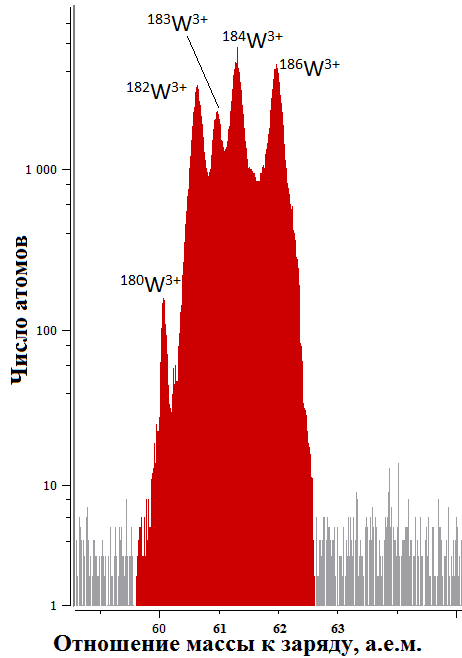
\includegraphics[width=.5\textwidth]{W_massspectr}
	}
	\caption{Масс-спектр образца из вольфрама}
	\label{fig:W_massspectr}
\end{figure}

Для оценки расстояния между атомными плоскостями были взяты отдельные части 3D объема в местах выхода кристаллографических направлений. Области выхода кристаллографических направлений определялись по двумерной гистограмме распределения событий на детектирующей системе, собранных за некоторый промежуток времени (Рисунок \cref{fig:W_3D}).

\begin{figure}[htb]
	\centerfloat{
		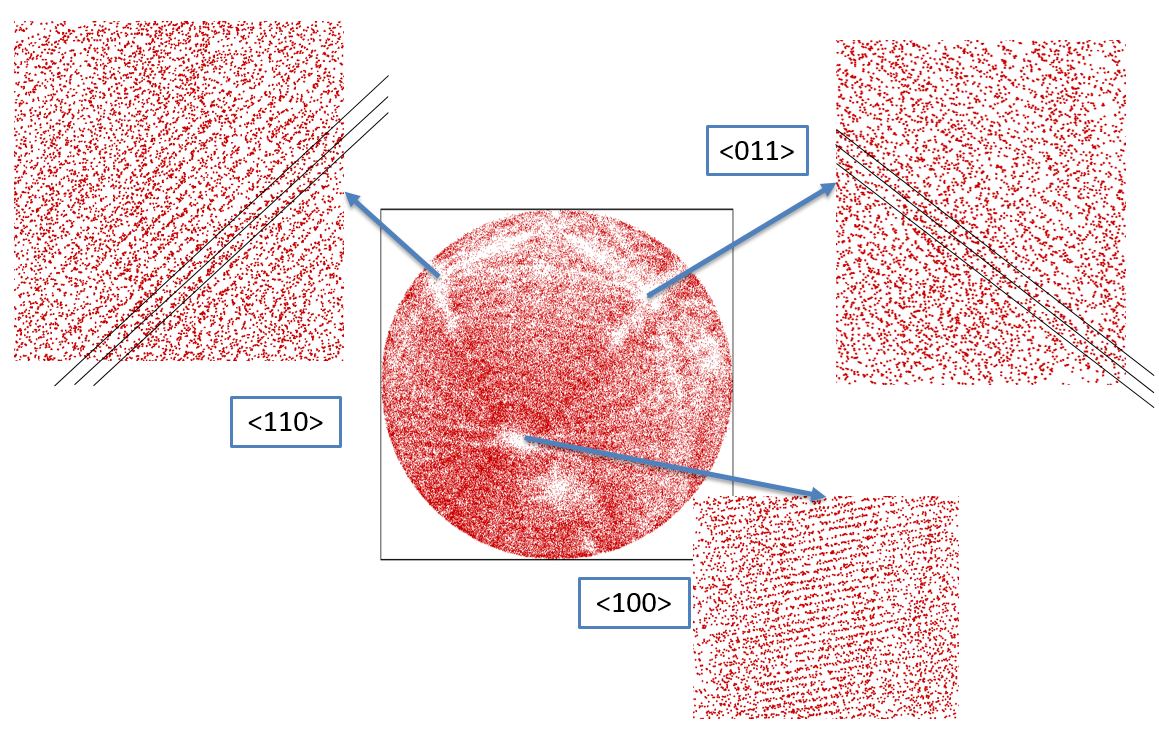
\includegraphics[width=\textwidth]{W_3D}
	}
	\caption{2D гистограмма распределения задетектированных событий}
	\label{fig:W_3D}
\end{figure}

Для каждого набора атомных плоскостей было определено среднее межплоскостное расстояние. Для выхода направления (100) измеренное расстояние составило 1.58 $\pm$ 0.03 \r{А}, что совпадает с табличным значение для вольфрама 1.58 \r{A} в переделах погрешности. Поскольку в данных исследованиях выход (100) ориентирован вдоль оси образца, то способность установки наблюдать атомные плоскости позволяет оценить разрешающую способность прибора вдоль оси образца (Z) в не более чем 1-2 \r{A}. Для выходов (011) также было измерено межплоскостное расстояние: 1.9 $\pm$ 0.3 \r{A}, что также согласуется с табличным значением в 2.2 \r{A}. Наборы плоскостей (011) и (110) расположены под углом к оси образца, это позволяет оценить латеральное разрешение установки: 2-4 \r{A}. Полученные оценки разрешающей способности ПАЗЛ-3D  характерны для большинства атомно-зондовых томографов. 

\FloatBarrier

\section{Определение оптимальной метрики качества испарения}\label{sec:ch3/sect3}

В ходе сбора данных с одного образца ряд факторов может приводить к изменению условий испарения атомов материала. Например, происходит изменение формы кончика образца (так как он постепенно испаряется), может происходить медленный <<дрейф>>  мощности лазера или фокусировка лазерного излучения может выйти из оптимального положения. Данные изменения приводят к различным отклонениям в испарении, которые будут влиять на результат анализа данных. Следовательно, для проведения количественных исследований необходимо разработать методику поддержания постоянных и воспроизводимых условий испарения в рамках исследования одного образца. В разделе \cref{sec:ch1/sec5} описаны основные используемые метрики для сравнения АЗТ данных. Поскольку ПАЗЛ-3D это новая разработанная установка, то необходимо разработать методику сравнения результатов исследований для обеспечения воспроизводимости получаемых данных.

Для отработки данной методики был выбран сплав Al-3.5Cu-0.2Mn-0.1S~wt\%. Это однородный материал на масштабах нескольких сотен нанометров. Также стоит отметить, что это 4-компонентный сплав, что дает возможность проследить изменения концентраций нескольких элементов друг относительно друга при различных условиях испарения. Исследования проводились при постоянной температуре образца 50 К. Остальные параметры менялись в ходе сбора данных. В начале работы были выбраны несколько различных метрик-кандидатов для оценки пригодности для контроля условий испарения. Ниже приведен список возможных метрик:

\begin{itemize}
	\item Концентрации элементов,
	\item Мощность лазерного излучения,
	\item Доля однократных событий (или общая доля мультисобытий),
	\item Доля мультисобытий одного из элементов,
	\item Соотношение зарядностей основного элемента,
	\item Доля шум до пика основного элемента (10-11 а.е.м.),
	\item Доля шум после пика основного элемента (40-41 а.е.м.).		
\end{itemize}

К метрикам предъявлялось несколько требований. Первое и основное - корректность получаемых концентраций элементов. Второе, не менее важное требование, это возможность вычислять значение выбранной метрики <<in-situ>> в процессе сбора данных. Также требовалась минимальная повторяемость результатов, хотя бы в рамках одного исследования. Для оценки повторяемости значений метрик данные собирались в определенном порядке. Основным варьируемым параметром являлась мощность лазерного излучения. Соответственно, в ходе исследований мощность сначала поэтапно уменьшали, потом увеличивали, затем опять уменьшали. Это позволило оценить возможность воспроизводить условия испарения на протяжении всего сбора данных. В таблицах Приложения \cref{app:B} приведены все параметры проведения исследований и результаты расчета значений выбранных метрик. Далее в работе показаны основные зависимости, которые были обнаружены или наличие которых было подтверждено (ранее они описывались для других атомно-зондовых томографов).

Наиболее очевидной и ожидаемой являлась зависимость детектируемой концентрации от мощности лазерного излучения. Точки зависимости приведены на Рисунках  \cref{fig:params_Conc_Power}, где точки соединены в порядке сбора данных.  Зависимость концентрации элемента практически прямо пропорциональна мощности лазерного излучения. Но в случае другой фокусировки лазера, а следовательно и другой мощности излучения лазера, уже наблюдается нелинейная зависимость (рисунок \cref{fig:params_Conc_Power} б)). Скорее всего есть область оптимума точности сбора данных между слишком малой и слишком большой мощностями лазерного излучения. Данное предположение коррелирует с наблюдаемыми зависимостями качества данных в работе \cite{scbibOptParamsYAFI} (подробно описывалось в разделе \cref{sec:ch1/sec5}).

\begin{figure}[htb]
	\begin{minipage}[b]{0.49\textwidth}\centering
		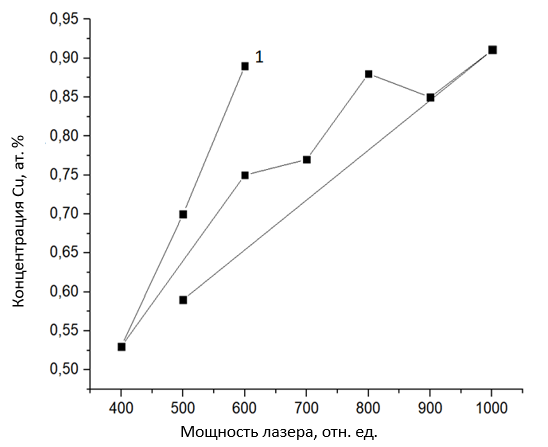
\includegraphics[width=\textwidth]{params_Conc_Power} \\ а)
	\end{minipage}
	\begin{minipage}[b]{0.49\textwidth}\centering
		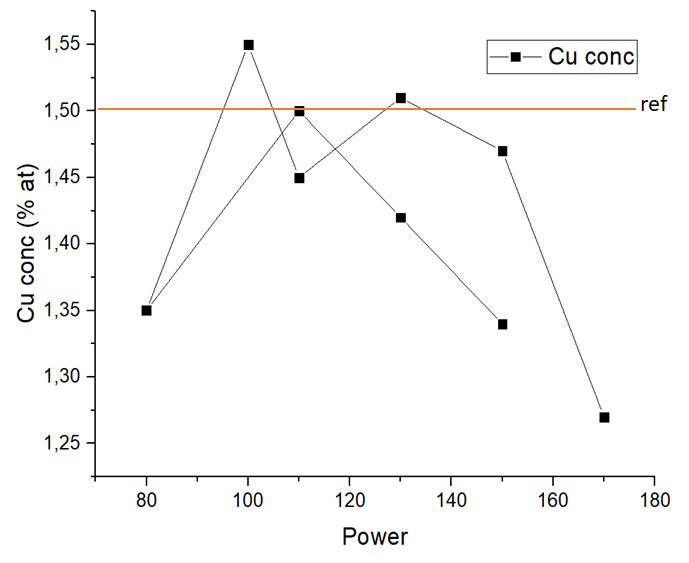
\includegraphics[width=\textwidth]{params_Conc_Power_2} \\ б)
	\end{minipage}
	\caption{Значения концентрации Cu при различной мощности лазерного излучения для двух наборов исследований. Точки соединены в порядке сбора данных. Оранжевой горизонтальной линией на отмечено табличное значение концентрации меди для исследуемого материала}
	\label{fig:params_Conc_Power}
\end{figure}

\FloatBarrier

Важно отметить, что данные для Рисунка \cref{fig:params_Conc_Power} были обработаны уже после проведения исследований. Как выше было неоднократно отмечено, что напрямую концентрации в процессе сбора данных затруднительно вычислять точно, с учетом шума/коррекций/оптимизаций.

Далее изучим другую, более перспективную метрику, основанную на соотношении зарядностей. Поскольку основным элементом в данном материале является алюминий, то была оценена зависимость концентрации меди от отношения $Al^{+}/Al^{++}$ (Рисунок \cref{fig:params_Conc_CSR}).

\begin{figure}[htb]
	\begin{minipage}[b]{0.49\textwidth}\centering
		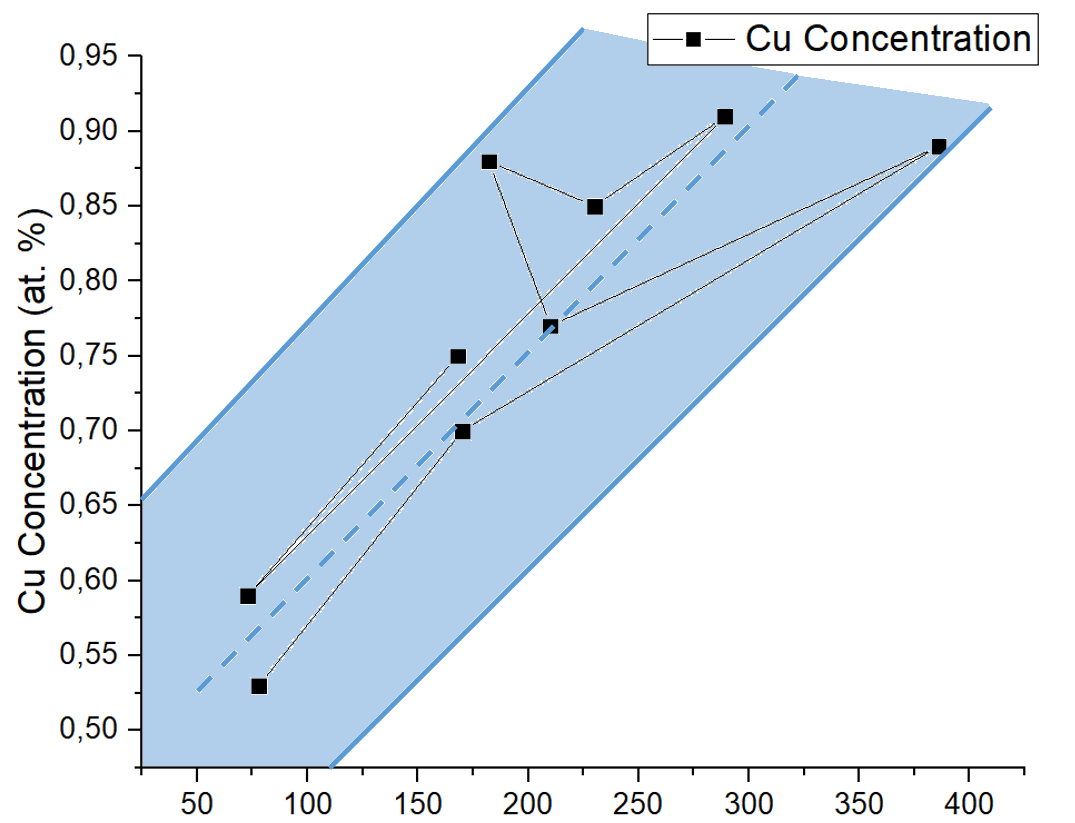
\includegraphics[width=\textwidth]{CSR_1} \\ а)
	\end{minipage}
	\begin{minipage}[b]{0.49\textwidth}\centering
		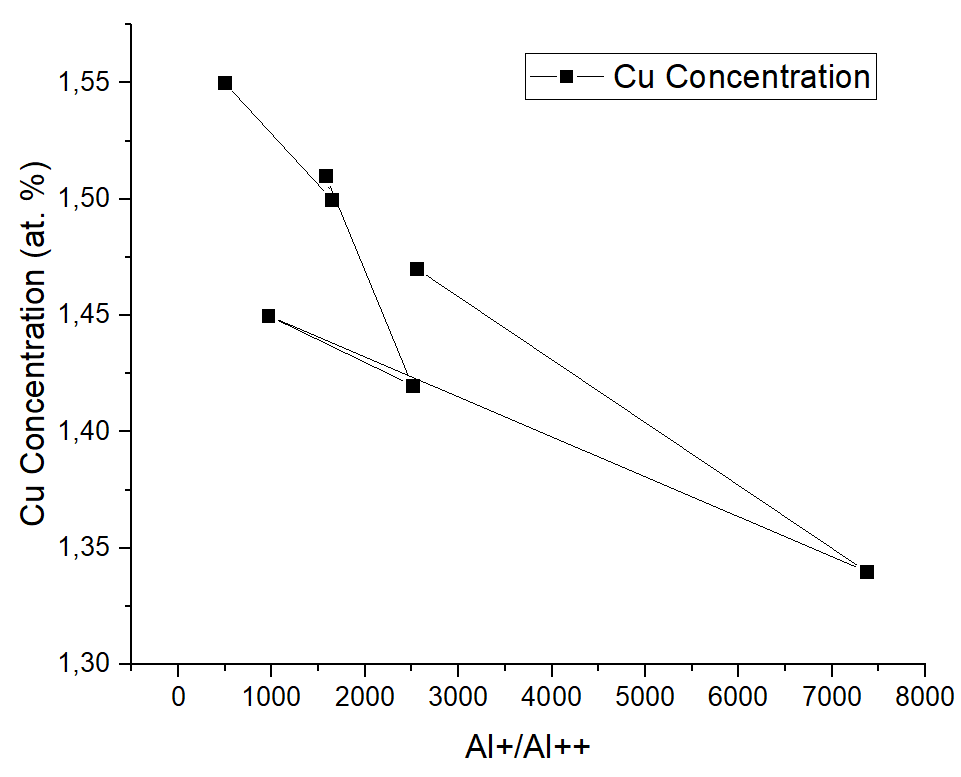
\includegraphics[width=\textwidth]{CSR_2} \\ б)
	\end{minipage}
	\caption{Значения концентрации Cu при различном соотношении зарядностей алюминия для двух наборов исследований. Точки соединены в порядке сбора данных.}
	\label{fig:params_Conc_CSR}
\end{figure}

На Рисунке \cref{fig:params_Conc_CSR} наглядно видно, что для первого набора данных в области значений $Al^{+}/Al^{++}$ от 75 до 400 концентрация меди не достигает требуемого значения в 1.52 ат. \%, но при этом явно наблюдается воспроизводимость значения концентрации при похожих значениях соотношения зарядностей. Наблюдаемую зависимость можно аппроксимировать линейной функцией ($y = ax + b$) с параметрами a = XXX, b = YYYYY. При этом для второго набора данных наблюдается противоположный характер зависимости. В этом случае можно также провести аппроксимацию линейной зависимостью с параметрами a = XXX, b = YYYYY. Стоит отметить, что во втором наборе данных 2 промежуточные точки практически с идеальной точностью соответствуют табличному значению концентрации меди в данном материале. Аналогичный характер зависимостей наблюдался в работе \cite{Mancini14}, что подтверждает корректность предложенной методики. Для второго набора данных также построены значения концентраций других элементов  в зависимости от соотношения зарядностей алюминия ( Рисунок \cref{fig:params_Sn_Mn_O}).

\begin{figure*}
	\centering
	\begin{subfigure}[b]{0.475\textwidth}
		\centering
		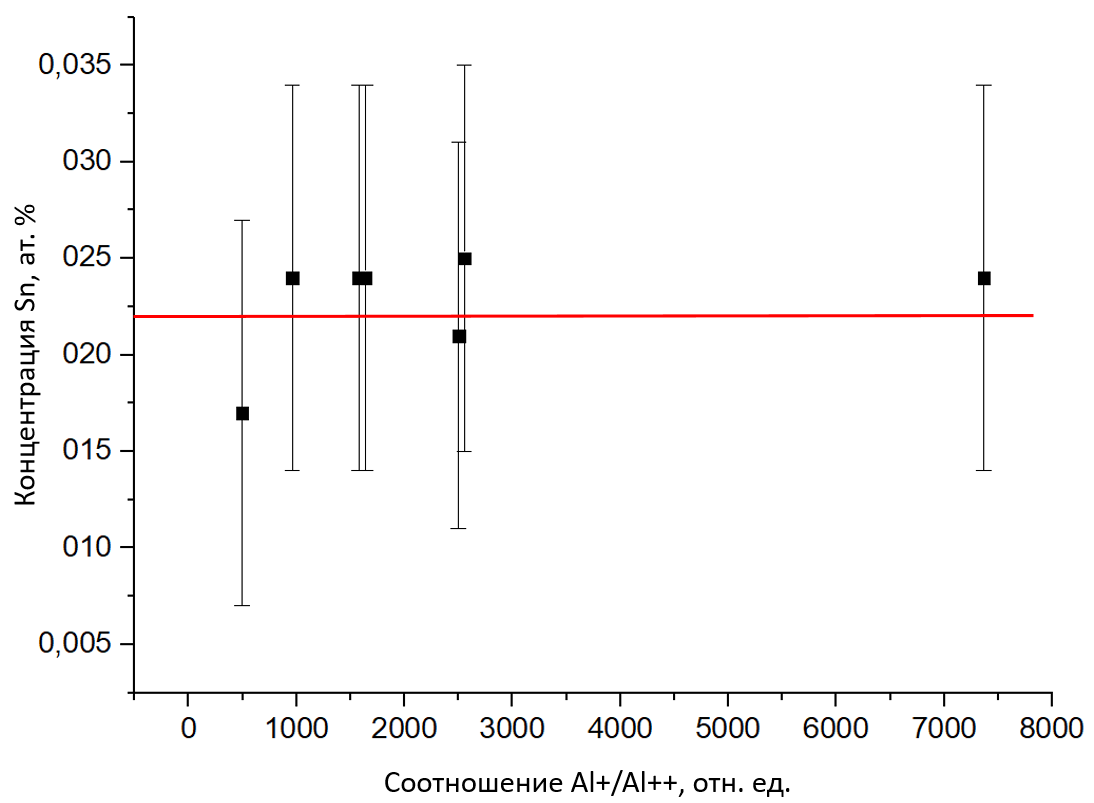
\includegraphics[width=\textwidth]{params_sn_conc}
		\caption{}    
	\end{subfigure}
	\hfill
	\begin{subfigure}[b]{0.475\textwidth}  
		\centering 
		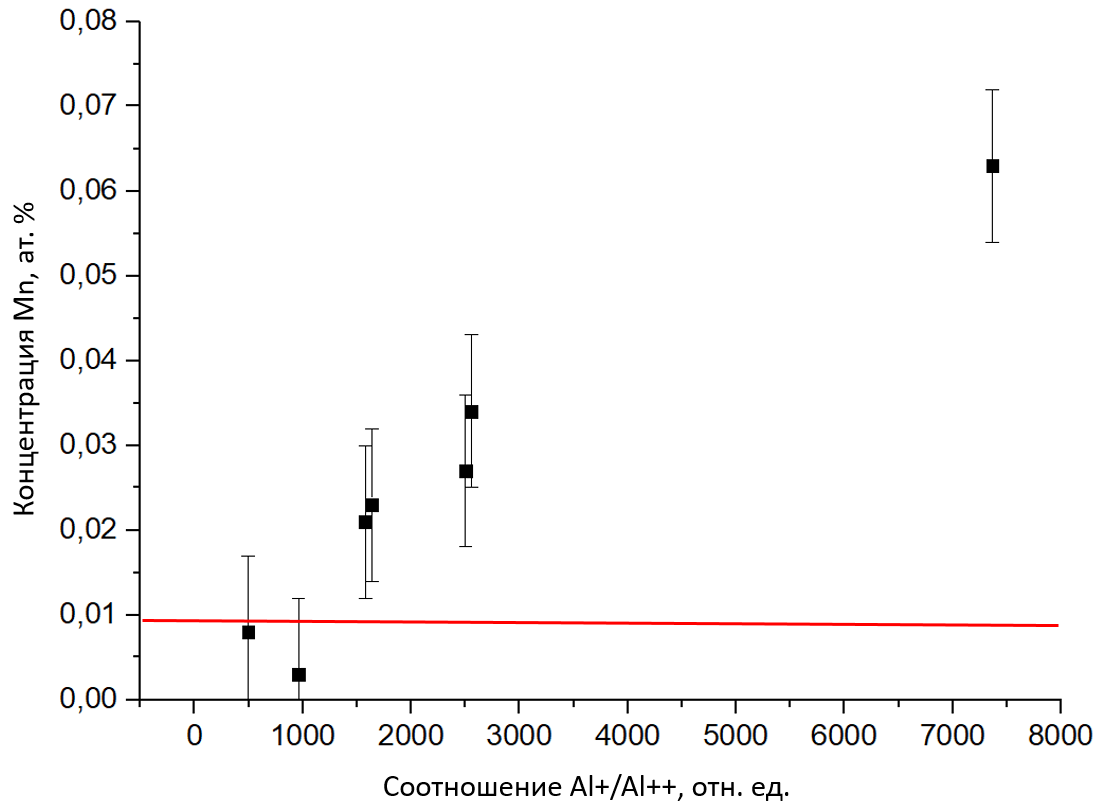
\includegraphics[width=\textwidth]{params_mn_conc}
		\caption{}    
	\end{subfigure}
	\vskip\baselineskip
	\begin{subfigure}[b]{0.475\textwidth}   
		\centering 
		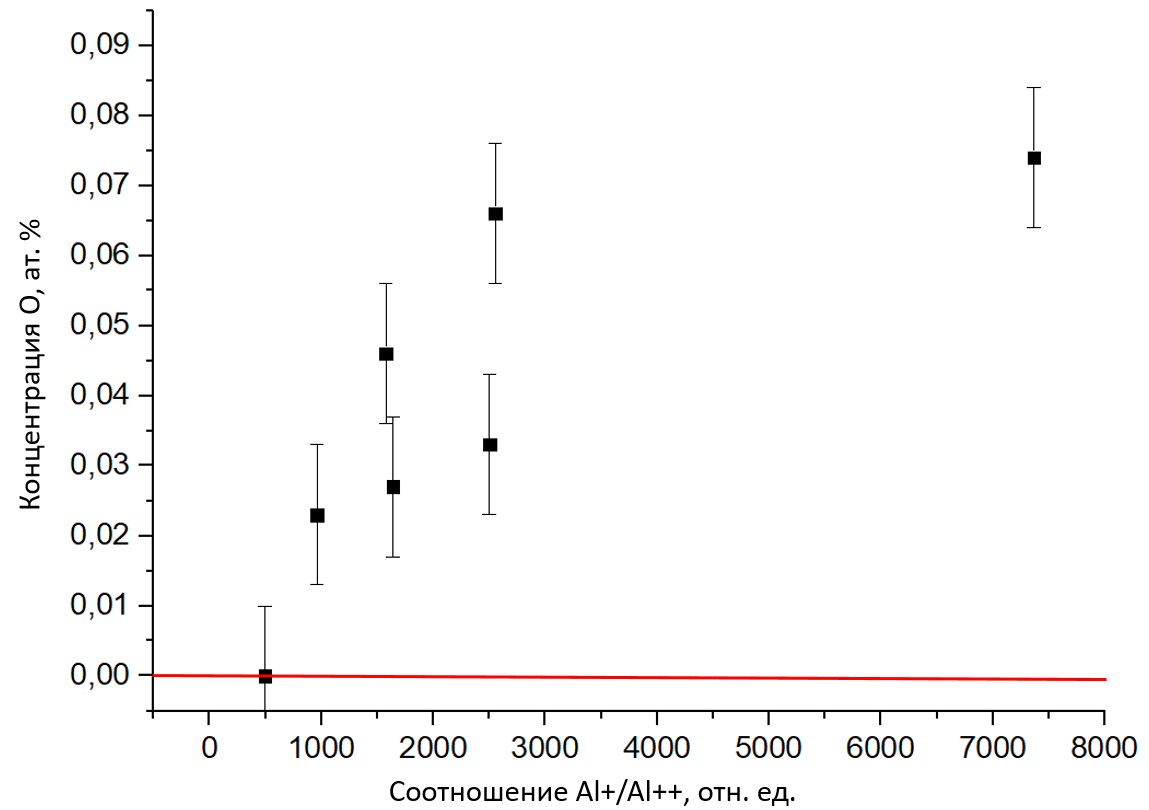
\includegraphics[width=\textwidth]{params_o_conc}
		\caption{}    
	\end{subfigure}
	\hfill
	\caption
	{Значения концентраций Sn (а), Mn (б), O (в) в зависимости от соотношения зарядностей алюминия. Красной линией указаны ожидаемые значения концентрации для исследуемого материала   } 
	\label{fig:params_Sn_Mn_O}
\end{figure*}

Анализируя результаты, показанные на Рисунках \cref{fig:params_Conc_CSR,fig:params_Sn_Mn_O} можно заключить, что для установки ПАЗЛ-3D для алюминиевого сплава Al-3.5Cu-0.2Mn-0.1S~wt\% оптимальным диапазоном значений соотношения зарядностей является промежуток от 300 до 2000 отн. еди. В данном промежутке концентрации меди и олова наиболее близки к табличным значениям. При этом наблюдается малое количество кислорода, наличие которого является артефактом лазерного испарения. Таким образом показано, что соотношение зарядностей основного элемента может служить метрикой качества данных. Показана воспроизводимость результатов исследований с использованием контроля условий испарения по соотношению зарядностей основного элемента.

При оценке зависимости качества АЗТ данных от других метрик было продемонстрировано несколько второстепенных зависимостей (или показано их отсутствие) для сплава Al-3.5Cu-0.2Mn-0.1S~wt\%:

\begin{itemize}
	\item Доля мультисобытий не является воспроизводимой метрикой для АЗТ данных,
	\item Мощность лазерного излучения пропорциональная соотношению зарядностей, но имеет плохую воспроизводимость на разных наборах данных, а следовательно точно не подходит для разных установок (Рисунок \cref{fig:params_Noise_Multi} в)),	
	\item Доля мультисобытий меди имеет тенденцию к снижению с ростом напряжения на образце,
	\item Доля шум до пика основного элемента (10-11 а.е.м.) и доля шум после пика основного элемента (40-41 а.е.м.)	падают с увеличением мощности лазерного излучения и увеличиваются с ростом напряжения на образце (Рисунок \cref{fig:params_Noise_Multi} а) и б)),
	\item Доля мультисобытий меди не является воспроизводимой метрикой для АЗТ данных.	
\end{itemize}

Полученные второстепенные зависимости могут быть важны для более оптимального выбора условий испарения в дальнейших работах по развитию методик исследования алюминиевых сплавов. Также полученные корреляции могут использоваться для лучшей интерпретации данных. Все указанные метрики собраны в Таблице \cref{tab:params_expl}, в которой также приведены основные их особенности как кандидатов для основной метрики качества и воспроизводимости данных.

\begin{figure*}
	\centering
	\begin{subfigure}[b]{0.475\textwidth}
		\centering
		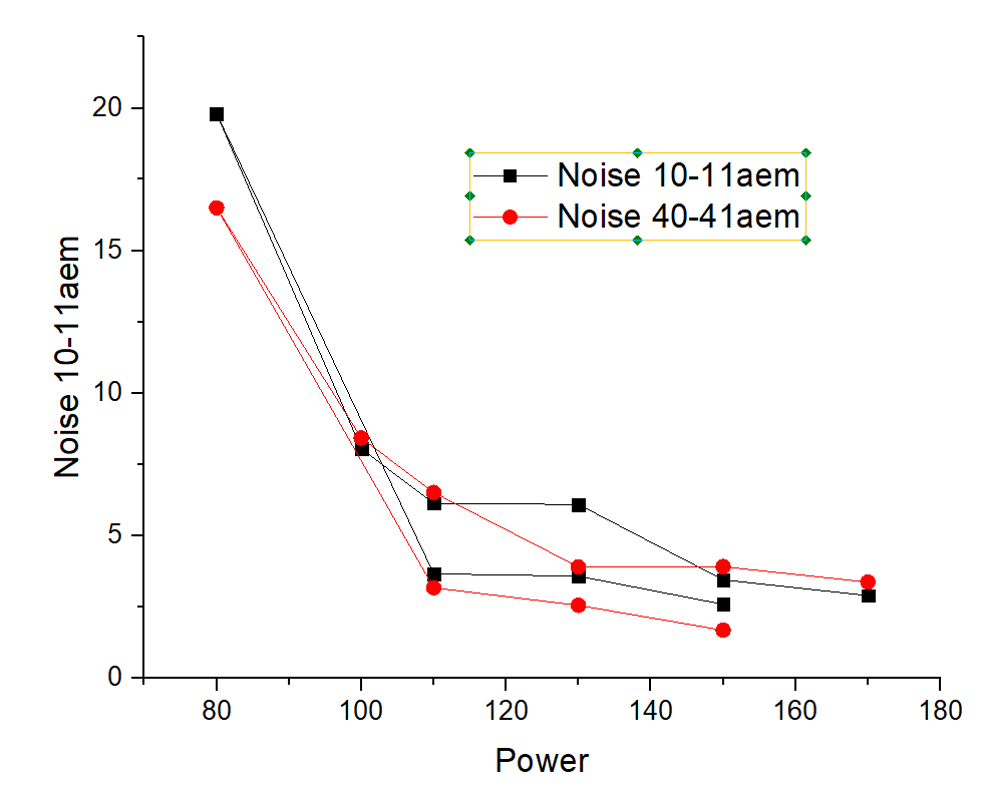
\includegraphics[width=\textwidth]{params_Noise_Power}
		\caption{}    
	\end{subfigure}
	\hfill
	\begin{subfigure}[b]{0.475\textwidth}  
		\centering 
		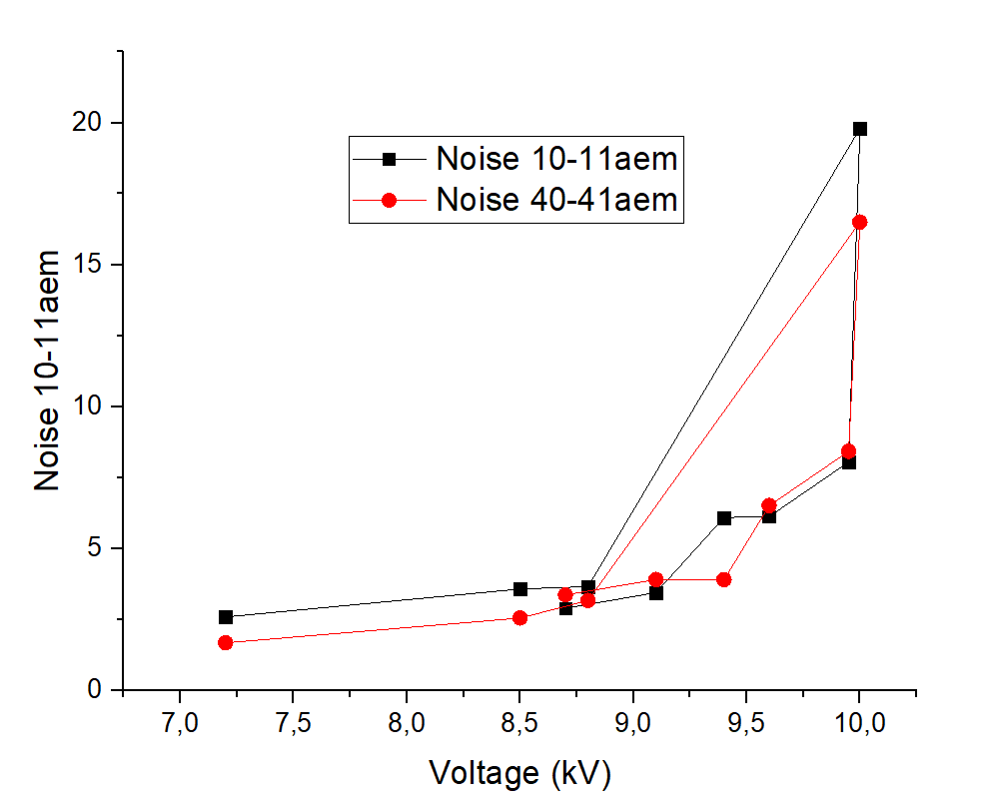
\includegraphics[width=\textwidth]{params_Noise_Voltage}
		\caption{}    
	\end{subfigure}
	\vskip\baselineskip
	\begin{subfigure}[b]{0.475\textwidth}   
		\centering 
		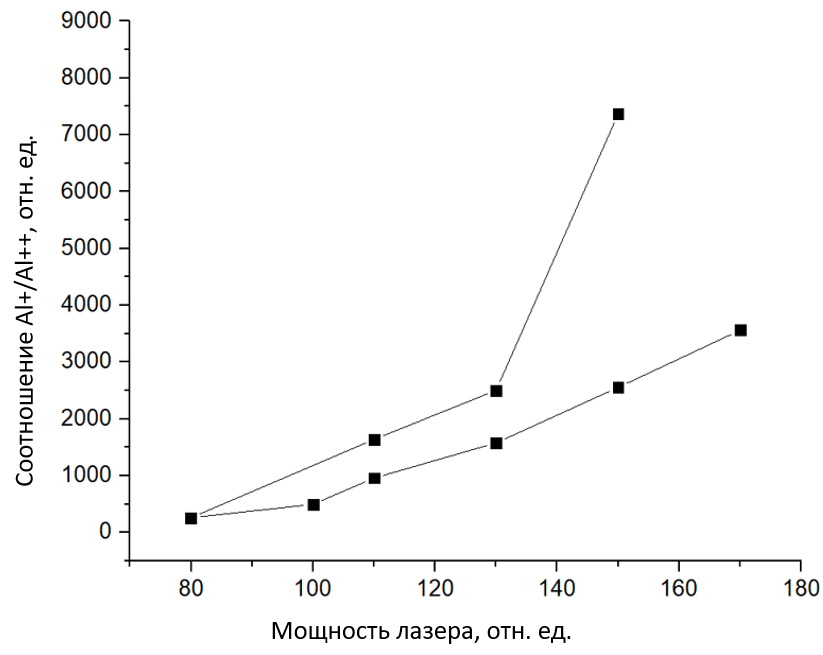
\includegraphics[width=\textwidth]{params_CSR_Power}
		\caption{}    
	\end{subfigure}
	\hfill
	\caption
	{а) - Значения шума до и после пика основного элемента от мощности лазерного излучения. б) - Значения шума до и после пика основного элемента от напряжения на образце. в) Значения соотношения зарядностей в зависимости от мощности лазерного излучения. На всех рисунках точки соединены в порядке сбора данных} 
	\label{fig:params_Noise_Multi}
\end{figure*}

\begin{table} [htb]
	\centering
	\caption{Метрики качества атомно-зондовых данных}
	\label{tab:params_expl}
	\begin{SingleSpace}
		\begin{tabularx}{\textwidth} {| X | X | X | X |}
			\hline
			Наименование & Описание/ комментарии & Возможная интерпретация & Минусы  \\ \hline
			Однократные события & {Доля однократных событий ко всем событиям}  & {Чем больше - тем проще расшифровывать данные}  & {Нет прямой корреляции с концентрациями}              \\ \hline
			Мощность лазера & {Легко измеряется/ меняется в процессе исследования}  & {-}  & {нет повторяемости от образца к образцу}              \\ \hline
			Доля мультисобытий Cu & Возможная метрика сложности точности определения концентрации & Чем меньше - тем лучше & Нет прямой корреляции с концентрациями          \\ \hline		
			Шум до пиков основного элемента сплава      & Доля атомов с массами от 10 до 11 а.е.м. & Чем больше мощность лазера, тем меньше шума, чем выше напряжение, тем больше шума  & Нет прямой корреляции с концентрациями               \\ \hline
			Шум после пиков основного элемента сплава     & Доля атомов с массами от 40 до 41 а.е.м. & Чем больше мощность лазера, тем меньше шума, чем выше напряжение, тем больше шума  & Нет прямой корреляции с концентрациями             \\ \hline
			Концентрации  & -   &  -   & Расчет невозможен в реальном времени  \\ \hline			
			Соотношение зарядностей основного элемента Al$^+$/Al$^{++}$, отн. ед.    & Возможна оценка по предварительному масс-спектру, без оптимизации   & Есть значимая зависимость и повторяемость концентраций от соотношения зарядностей  & Может отличаться для разных материалов   \\ \hline
		\end{tabularx}
	\end{SingleSpace}
\end{table}

\FloatBarrier
Таким образом, в данном разделе продемонстрирована методика выбора метрики качества и воспроизводимости АЗТ данных для алюминиевых сплавов. Показано, что предпочтительная метрика, основанная на соотношение зарядностей для основного химического элемента материала. Основываясь на том, что сохранение соотношения зарядностей основного химического элемента обеспечивают воспроизводимость результатов АЗТ исследований (концентрации близки к ожидаемым), можно заключить, что методика поиска оптимальных параметров испарения включает следующее:

\begin{itemize}
	\item сбор набора АЗТ данных при различных соотношения зарядностей основного химического элемента,
	\item расчет концентрации всех элементов,	
	\item (дополнительно) проверка данных на отсутствие артефактов испарения (например, наличия кислорода, не входящего в состав материала),
	\item в случае неполучения целевых значений концентраций или наличия большого числа артефактов проверка более широкого диапазона значений соотношений зарядностей,
	\item выбор диапазона значений соотношений зарадностей, при котором концентрации наиболее близки к целевым значениям и при этом наблюдается минимальное количество артефактов испарения.	
\end{itemize}
В дальнейших исследованиях сплавов данного типа можно придерживаться выбранного диапазона значений соотношений зарядностей.

\FloatBarrier

\section{Сравнение атомно-зондовых данных, полученных на установках ПАЗЛ-3D и АТЛАЗ на примере сплава Al-Cu-Zr}\label{sec:ch3/sect4}

Для демонстрации методики сравнения АЗТ данных, описанной в предыдущем разделе \cref{sec:ch3/sect3} было проведены исследования на двух АЗТ установках с лазерным испарением ПАЗЛ-3D и АТЛАЗ (Модернизированная АЗТ установка АТЛАЗ была собрана на базе прибора CAMECA ECOTAP). Для исследования выбирались материалы содержащие различные наноразмерные кластеры. Одним из материалов была выбрана сталь 16Х12МВСФБР ЭП-823 \cite{Porollo04} после облучения ионами (далее ЭП-823). Данная сталь отличается высокой плотность кластеров. Вторым материалом для сравнения выбран алюминиевый сплав Al-3.3Cu-2.5Mn-0.5Zr (мас. \%) после отжига при температурах 350 \textdegree С и 450 \textdegree С \cite{Belov22,Belov21} (далее сокращенно называются как Al-Cu-Mn-Zr 350 \textdegree С и Al-Cu-Mn-Zr 450 \textdegree С, соответственно). Основной задачей данного сравнения было демонстрация работоспособности методики, описанной в предыдущем разделе, для других материалов. Стоит отметить, что данная проверка проводилась для материалов без больших особенностей (большими считаются особенности структуры более 1 мкм). 

Поскольку данные исследования проводились на стадии отработки методики, то контролировалось больше технических параметров исследования, чем это было бы необходимо для обычных исследований <<на поток>>. В качестве метрик сравнения исследований использовались как общепринятые параметры, так и ряд технических характеристик данных, которые в обычных исследованиях используются редко. Обычно при анализе АЗТ данных в результатах приводятся концентрации химических элементов в матрице материала, в концентрации в кластерах, размеры кластеров и их объемная плотность. В данных исследованиях к этим метрикам был добавлен ряд таких параметров как: соотношение зарядностей основного элемента, разрешение по массе на полувысоте пика, разрешение по массе на 10~\% высоты пика, общий процент мульти-событий, доля мульти-событий, приходящаяся на элементы, которые являются кластеро-/фазо-образующими, скорость детектирования и уровень шума. Сравнение количества шума проводилось на участках масс-спектра после пиков основных элементов и сопоставлялось с учетом нормирования на общее число собранных атомов. В таблицах \cref{tab:paramsAPPLEvsATLAS,tab:matrixAPPLEvsATLAS,tab:clustersAPPLEvsATLAS}, представлено сравнение значений метрик на разных установках для алюминиевого сплава.

\begin{table} [htbp]
	\centering
	\caption{Сравнение характеристик точности восстановления данных для алюминиевых сплавов Al-Cu-Mn-Zr}
	\label{tab:paramsAPPLEvsATLAS}
	\begin{SingleSpace}
		\begin{tabular} {| c | c | c | c | c |}
			\hline
			{} & \thead{ПАЗЛ-3D, \\350 \textdegree C} & \thead{АТЛАЗ, \\350 \textdegree C} & \thead{ПАЗЛ-3D, \\450 \textdegree C} & \thead{АТЛАЗ, \\450 \textdegree C} \\ \hline
			$M/\Delta M_{50\%}$ Al$^+$ & 670  & 260  & 421  & 430               \\ \hline
			$M/\Delta M_{10\%}$ Al$^+$ & 206  & 120  & 146  & 190               \\ \hline
			Мульти-события, \%         & 0.7  & 2.9  & 0.9  & 2.9               \\ \hline
			Мульти-события Cu, \%      & 4.23 & 0.54 & 7.11 & 3.17              \\ \hline
			Мульти-события Zr, \%      & 7.31 & 0.85 & 0.18 & 0.6               \\ \hline
			Шум, 10$^{-5}$ отн. ед. & 5.4   & 1.9   & 10.7  & 1.67  \\ \hline
			Скорость сбора данных, атомов/возд.        & 0.005 & 0.006 & 0.007 & 0.007 \\ \hline
			Соотношение Al$^+$/Al$^{++}$, отн. ед.    & 640   & 310   & 630   & 450   \\ \hline
		\end{tabular}
	\end{SingleSpace}
\end{table}

Образцы из алюминия для АЗТ исследования были изготовлены с помощью электроэрозионной резки, с последующим электрохимическим утонением. В процессе сбора данных температура образцов поддерживалась равной 50~К. Мощность лазера на  ПАЗЛ-3D составляла 85 $\pm$ 1 мВт, а на АТЛАЗ - 3.0 $\pm$ 0.5 мВт. Скорость сбора данных представлена в Таблице \cref{tab:paramsAPPLEvsATLAS}. Обработка и восстановление АЗТ данных проводилась с помощью ПО <<КВАНТМ-3D>>. Параметры 3D восстановления были выбраны с помощью методики, описанной в работе \cite{scbibDensity}. Полевой фактор $k_f$ для всех исследований находится в диапазоне от 4 до 6, коэффициент сжатия изображения ICF  - от 1.2 до 1.6. Масс-спектр восстанавливался по методике, представленной в работе \cite{Shutov19}. Концентрации и их погрешности был для всех исследований были рассчитаны по формулам, предложенным в работах Danoix \cite{Danoix071,Danoix072}. В случае, если на одно состояние приходилось более одного исследования, то в качестве погрешности указано среднее отклонение от среднего значения. Состав кластеров определялся с помощью изо-концентрационных поверхностей, так как форма частиц сильно отличается от сферической (стандартный алгоритм определения размеров частиц может работать некорректно). Были выбраны следующие параметры построения из-концентрационных поверхностей: шаг сетки составлял от 1 до 1.5 нм, радиус делокализации равен 2 нм, пороговое значение концентрации Zr не менее 1.5 ат. \%.

\begin{figure}[h!tb]
	\begin{minipage}[b][][b]{0.49\textwidth}\centering
		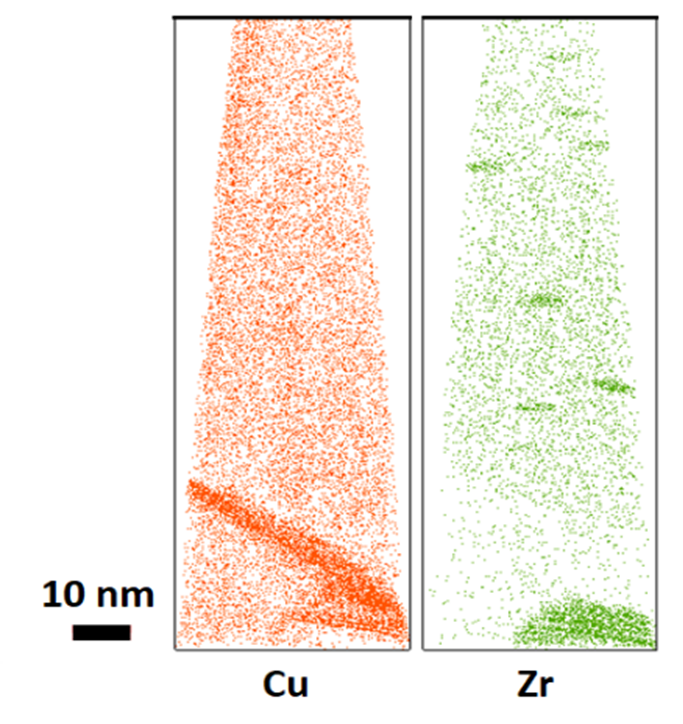
\includegraphics[scale=0.5]{APPLEvsATLAS_apple} \\ а)
	\end{minipage}
	%\hfill
	\begin{minipage}[b][][b]{0.49\textwidth}\centering
		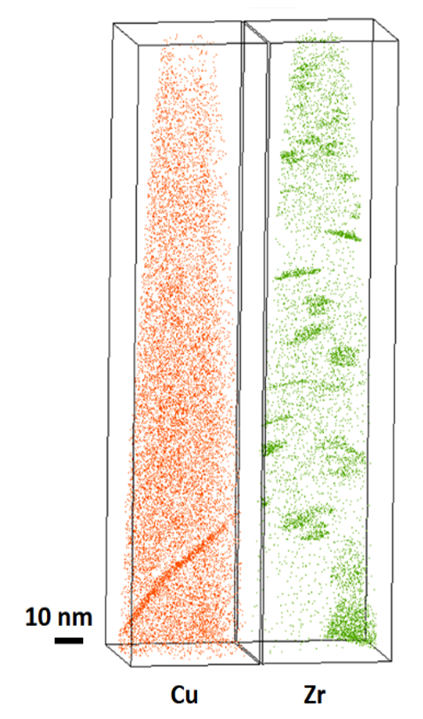
\includegraphics[scale=0.8]{APPLEvsATLAS_atlas} \\ б)
	\end{minipage}
	\caption{а) Атомные карты сплава Al-Cu-Mn-Zr 350~\textdegree C (ПАЗЛ-3D). б) Атомные карты сплава Al-Cu-Mn-Zr 350~\textdegree C (АТЛАЗ) \cite{scbibAPPLEvsATLAS}.}
	\label{fig:APPLEvsATLAS}
\end{figure} 

Атомные карты образцов из алюминиевого сплава Al-Cu-Mn-Zr 350~\textdegree C представлены на Рисунке \cref{fig:APPLEvsATLAS}. На обеих установках в область зрения попали границы зерен, декорированные медью. Для каждого состояния проведен расчет концентраций химических элементов в матрице (Таблица \cref{tab:matrixAPPLEvsATLAS}). В состоянии Al-Cu-Mn-Zr 350~\textdegree C были обнаружены кластеры Zr как с помощью ПАЗЛ-3D, так и с помощью АТЛАЗ. Состав кластеров для Al-Cu-Mn-Zr 350~\textdegree C показан в Таблице \cref{tab:clustersAPPLEvsATLAS}. 

\begin{table} [htbp]
	\centering
	\caption{Состав матрицы [ат. \%] в алюминиевом сплаве Al-Cu-Mn-Zr после отжига при 350~\textdegree C и при 450~\textdegree C \cite{scbibAPPLEvsATLAS}, полученный на установках ПАЗЛ-3D и АТЛАЗ}
	\label{tab:matrixAPPLEvsATLAS}
	\begin{SingleSpace}
		\begin{tabular} {| c | c | c | c | c |}
			\hline
			{} & \thead{ПАЗЛ-3D, \\ 350~\textdegree C} & \thead{АТЛАЗ, \\ 350~\textdegree C} & \thead{ПАЗЛ-3D, \\ 450~\textdegree C} & \thead{АТЛАЗ, \\ 450~\textdegree C} \\ \hline
			Al       & 99.49 $\pm$ 0.01  & 99.66 $\pm$ 0.01 & 99.2 $\pm$ 0.1  & 99.20 $\pm$ 0.01  \\ \hline
			Cu       & 0.29 $\pm$ 0.06   & 0.24 $\pm$ 0.04  & 0.6 $\pm$ 0.2  & 0.67 $\pm$ 0.05  \\ \hline
			Mn       & 0.01 $\pm$ 0.01 & 0.004 $\pm$ 0.002 & 0.02 $\pm$ 0.01  & 0.010 $\pm$ 0.005 \\ \hline
			Zr       & 0.11 $\pm$ 0.05   & 0.06 $\pm$ 0.04 & 0.010 $\pm$ 0.008  & 
			0.08 $\pm$ 0.05   \\ \hline
			Ni, C, O & Баланс & Баланс & Баланс & Баланс  \\ \hline			
		\end{tabular}
	\end{SingleSpace}
\end{table}

\begin{table} [htbp]
	\centering
	\caption{Состав кластеров [ат. \%] в алюминиевом сплаве Al-Cu-Mn-Zr после отжига при 350~\textdegree C \cite{scbibAPPLEvsATLAS}, полученный на установках ПАЗЛ-3D и АТЛАЗ}
	\label{tab:clustersAPPLEvsATLAS}
	\begin{SingleSpace}
		\begin{tabular} {| c | c | c |}
			\hline
			{} & ПАЗЛ-3D & АТЛАЗ \\ \hline
			Al       & 96.9 $\pm$ 0.3  & 96.7 $\pm$ 0.4   \\ \hline
			Cu       & 0.3 $\pm$ 0.1   & 0.3 $\pm$ 0.1    \\ \hline
			Mn       & 0.04 $\pm$ 0.02 & 0.003 $\pm$ 0.002  \\ \hline
			Zr       & 2.4 $\pm$ 0.3   & 2.8 $\pm$ 0.2    \\ \hline
			Ni, C, O & Баланс & Баланс   \\ \hline			
		\end{tabular}
	\end{SingleSpace}
\end{table}

Рассчитана плотность включений Zr для данных, полученных на ПАЗЛ-3D, составила (0.9 $\pm$ 0.1) x 10$^{23}$ и (1.40 $\pm$ 0.05) x 10$^{23}$ м$^{-3}$ для АТЛАЗ. Полученные значения плотности различаются менее чем на порядок. Поскольку на масштабах десятков и сотен нанометров плотность частиц может отличаться в зависимости от случайного выбора области исследования, то полученный результаты плотности можно считать достоверными. Полученные значения составов матриц и кластеров Zr для алюминиевых сплавов сходятся в пределах погрешностей, что говорит о правильности выбора характеристик, обеспечивающих контроль одинаковости условий испарения на разных установках.


\FloatBarrier

Втором материалом для сравнения использовалась сталь ЭП-823. Условия сбора данных были близки, к тем, что использовались при исследовании алюминиевых сплавов. Мощность лазерного излучения равна на АТЛАЗ - 2 $\pm$ 0.5 мВт, а на ПАЗЛ-3D - 40 $\pm$ 1 мВт. Восстановление координат и масс-спектра проводилось по тем же алгоритмам, что для алюминиевых сплавов. Коэффициент сжатия изображения был выбран в диапазоне от 1.2 до 1.35. Полевой фактор при этом равнялся 4.5. В отличии от алюминиевых сплавов, в сплаве на основе Fe-Cr есть изотопы разных элементов, атомные масс которых не разрешимы с помощью атомно-зондовой томографии. Для данного материал был проведен дополнительный расчет изотопных соотношений для изотопов Fe, Cr, Ni для учета перекрывающихся пиков изотопов. Поиск кластеров проводился с помощью алгоритма максимального разделения \cite{Vurpillot16}. Были использованы следующие параметры поиска кластеров для данных, полученных на ПАЗЛ-3D: радиус поиска R = 8, минимальное число атомов в сфере поиска $N_{min}$ = 7. Для данных, полученных на АТЛАЗ использовались следующие параметры: радиус поиска R = 7, минимальное число атомов в сфере поиска $N_{min}$ = 7.5. Технические характеристики полученных полученных данных показаны в Таблице \cref{tab:paramsAPPLEvsATLAS_EP3}. Радиус кластеров рассчитывался как радиус Гирации.

\begin{table} [htbp]
	\centering
	\caption{Сравнения характеристик точности восстановления данных для ЭП-823 на установках ПАЗЛ-3D и АТЛАЗ}
	\label{tab:paramsAPPLEvsATLAS_EP3}
	\begin{SingleSpace}
		\begin{tabular} {| c | c | c |}
			\hline
			{}                                     & ПАЗЛ-3D & АТЛАЗ   \\ \hline
			$M/\Delta M_{50\%}$ Al$^+$             & 938     & 726     \\ \hline
			$M/\Delta M_{10\%}$ Al$^+$             & 245     & 329     \\ \hline
			Мульти-события, \%                     & 1.4     & 17.7                 \\ \hline
			Мульти-события Ni, \%                  & 1.7     & 28.6             \\ \hline
			Мульти-события Si, \%                  & 0.4     & 26.1             \\ \hline
			Мульти-события Cu, \%                  & 3.9     & 6.7             \\ \hline
			Шум, 10$^{-5}$ отн. ед.                & 10.05   & 30.1     \\ \hline
			Скорость сбора данных, атомов/возд.    & 0.008   & 0.01  \\ \hline
			Соотношение Al$^+$/Al$^{++}$, отн. ед. & 307     & 368     \\ \hline
		\end{tabular}
	\end{SingleSpace}
\end{table}

На Рисунке \cref{fig:APPLEvsATLAS_EP} показаны атомные карты объемов стали ЭП-823, полученные на разных установках АЗТ. Полученные составы матрицы и кластеров представлены в Таблице \cref{fig:APPLEvsATLAS_EP}.

\begin{figure}[h!tb]
	\begin{minipage}[b][][b]{0.49\textwidth}\centering
		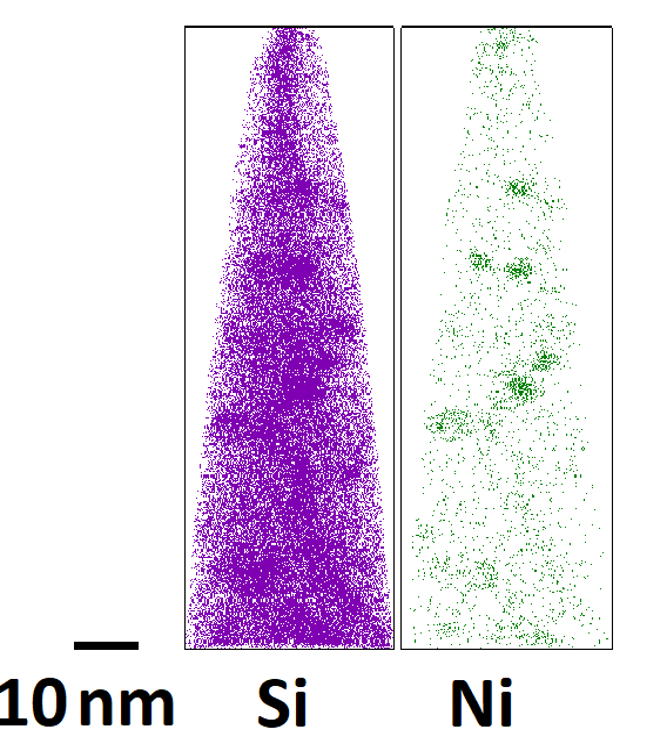
\includegraphics[scale=0.5]{APPLEvsATLAS_apple_EP} \\ а)
	\end{minipage}
	%\hfill
	\begin{minipage}[b][][b]{0.49\textwidth}\centering
		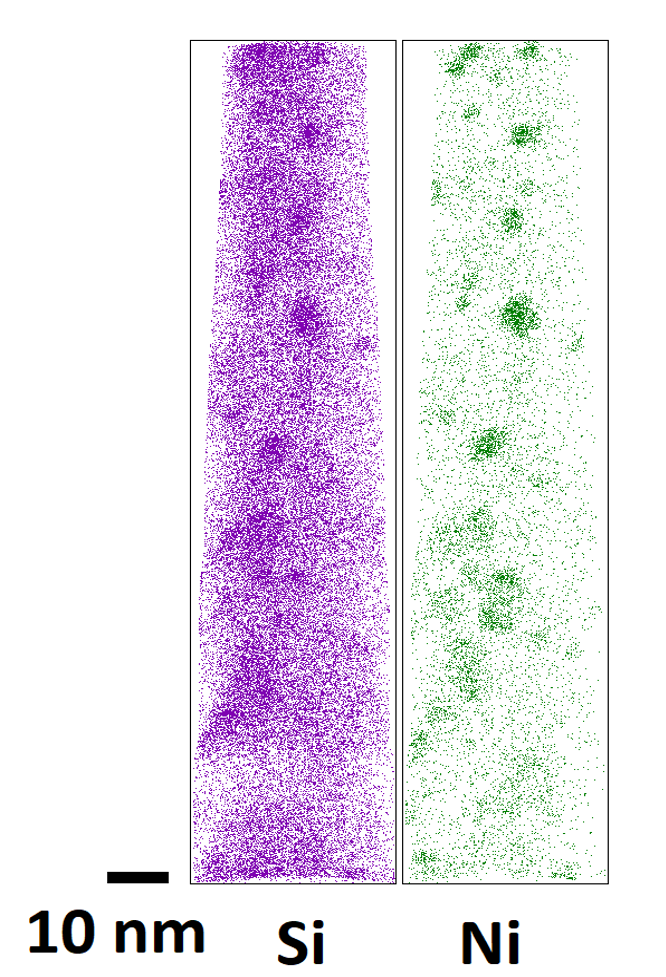
\includegraphics[scale=0.8]{APPLEvsATLAS_atlas_EP} \\ б)
	\end{minipage}
	\caption{Атомные карты \cite{scbibAPPLEvsATLAS} облученной стали ЭП-823 на ПАЗЛ-3D (а) и АТЛАЗ (б).}
	\label{fig:APPLEvsATLAS_EP}
\end{figure} 

\begin{table} [htbp]
	\centering
	\caption{Сравнение состава матрицы и кластеров [ат. \%] для стали ЭП-823 \cite{scbibAPPLEvsATLAS} после облучения, полученных на установках ПАЗЛ-3D и АТЛАЗ.}
	\label{tab:matrix_clustersAPPLEvsATLAS}
	\begin{SingleSpace}
		\begin{tabular} {| c | c | c | c | c |}
			\hline
			{} & \thead{ПАЗЛ-3D матрица} & \thead{АТЛАЗ матрица} & \thead{ПАЗЛ-3D кластеры} & \thead{АТЛАЗ кластеры} \\ \hline
			Fe       & 83.43 $\pm$ 0.02 & 83.98 $\pm$ 0.02  & 48 $\pm$ 1      & 53 $\pm$ 1  \\ \hline
			Cr       & 11.11 $\pm$ 0.06 & 10.51 $\pm$ 0.05  & 6.9 $\pm$ 0.8   & 7.3 $\pm$ 0.7   \\ \hline
			Si       & 2.59 $\pm$ 0.06  & 1.88 $\pm$ 0.05   & 15 $\pm$ 1      & 10.0 $\pm$ 0.8 \\ \hline
			Mn       & 0.94 $\pm$ 0.06  & 1.98 $\pm$ 0.05   & 4.5 $\pm$ 0,6   & 4.7 $\pm$ 0.5   \\ \hline
			Ni       & 0.59 $\pm$ 0.06  & 0.78 $\pm$ 0.05   & 23 $\pm$ 1      & 21 $\pm$ 1   \\ \hline
			Cu       & 0.05 $\pm$ 0.04  & 0.08 $\pm$ 0.05   & 0.2 $\pm$ 0,1   & 0.5 $\pm$ 0.2   \\ \hline
			W        & 0.16 $\pm$ 0.06  & 0.28 $\pm$ 0.05   & 0.03 $\pm$ 0,03 & 0.2 $\pm$ 0.1   \\ \hline
			C        & 0.08 $\pm$ 0.06  & 0.09 $\pm$ 0.05   & 0.11 $\pm$ 0,06 & 0.08 $\pm$ 0.06   \\ \hline
			Nb       & 0.07 $\pm$ 0.06  & -                 & 0.3 $\pm$ 0.1   & 0.5 $\pm$ 0.1   \\ \hline
			Остальные & Баланс & Баланс & Баланс & Баланс               \\ \hline			
		\end{tabular}
	\end{SingleSpace}
\end{table}

Средний радиус кластеров составил (2.8 $\pm$ 0.2) нм и (3.2 $\pm$ 0.4) нм для ПАЗЛ-3D и АТЛАЗ, соответственно. Значения среднего радиуса кластеров совпадают для данных, полученных на обеих установках. Средние значения плотности кластеров в объеме также совпадают в переделах погрешности: (1.2 $\pm$ 0.4) x 10$^{23}$ и (1.1 $\pm$ 0.2) x 10$^{23}$ м$^{-3}$ для ПАЗЛ-3D и АТЛАЗ, соответственно. Составы матриц и кластеров имеют незначительные отличия. При этом набор химических элементов в составе кластеров, по которым обогащены кластеры, одинаков на обеих установках. Небольшие различия в значениях концентраций некоторых элементов могут быть вызваны неоднородностью материала после облучения.

По результатам сравнения можно заключить, что выбор установки для исследования материала незначительно влияет на качество получаемых данных. Если данные были собраны при близких значениях 

(ПЕРЕПИСАТЬ ниже )















Как видно из полученных выше характеристик точности восстановления данных установки ПАЗЛ-3D и АТЛАЗ сравнимы по разрешению по массе и для алюминиевых сплавов, и для сталей. Количество шума при исследовании алюминиевого сплава отличается в 3-6 раз в пользу АТЛАЗ, но в случае со сталью ситуация противоположная (на АТЛАЗ шума больше в три раза). Данный факт вызван скорее разными условиями испарения образцов – разная скорость сбора данных и неодинаковая форма образцов. Наблюдаются общие закономерности при сравнении доли мульти-событий. На АТЛАЗ детектируется существенно больше мульти-событий, чем на ПАЗЛ-3D. В случае исследования чистых материалов или алюминиевых сплавов это практически не играет роли. При исследовании стали получены данные с 17.7 \% мульти-событий. Предположительно, это может быть вызвано использованием криогенной системы без устройств гашения вибраций на АТЛАЗ (вибрации могут составлять более 20 мкм), на которую непосредственно закреплен держатель образца. Это может приводить к частому выходу образца из области освещения лучом лазера, что влечет за собой необходимость поддерживать более высокую интенсивность испарения в моменты корректного освещения вершины образца. Известно, что в этом случае количество мульти-событий возрастает, и снижается точность химической идентификации \cite{scbibOptParamsYAFI}. Различия в пропорции между элементами в мульти-событиях для алюминиевых сплавов, как видно из результатов, не вносит существенного различия в определяемый химический состав матрицы и кластеров. Скорее всего, отсутствие разницы обусловлено малым значением общего числа мульти-событий. Для ЭП-823, при исследовании на АТЛАЗ, получены существенно большие значения мульти-событий как для общее числа, так в пропорциях по элементам. Как следствие, наблюдаются отличия по концентрациям для Si, Mn, W и Cr, что, скорее всего, может быть нивелировано более точным подбором условий испарения или модернизацией прибора за счет уменьшения вибраций держателя образца.

Сравнение результатов исследования вольфрама позволяет заключить, что установки имеют практически идентичное пространственное разрешение 1-4 \r{A}. Это позволяет предположить, что все пространственные характеристики при сравнении данных должны быть иметь мало различий между установками. Данный тезис подтверждается при сравнении среднего размера кластеров в стали ЭП-823 и преципитатов Zr в алюминиевом сплаве. В обоих случаях средний размер нано-размерных объектов совпадает в пределах статистической погрешности. С другой стороны, в сплаве Al-Cu-Mn-Zr 350°С на разных установках наблюдается некоторое отличие рассчитанной плотности кластеров. Ввиду небольшой разницы результатов (всего в 1.5 раза) можно предположить, что причина отклонения в плотности частиц связана с реальными различиями плотности в разных зернах материала. При этом химический состав как матрицы, так и частиц для алюминиевых сплавов совпадает в пределах погрешности.

(ПЕРЕПИСАТЬ выше )

\FloatBarrier

\section{Методика коррекции восстановления атомно-зондовых данных с учетом атомной плотности}\label{sec:ch3/sect5}

В атомно-зондовой томографии на качество данных влияет множество факторов на каждом из этапов работы с данными. В ходе сбора данных на установке необходимо следовать определенным методикам сбора данных (например, см. Раздел \cref{sec:ch3/sect4}). Восстановление АЗТ данных также является сложной процедурой, которая может существенно повлиять на количественные характеристики результатов исследования. На точность восстановления 3D координат атомов в АЗТ данных зависит от параметров и конфигурации АЗТ установки и от алгоритма восстановления координат. Для реконструкции 3D координат можно использовать несколько алгоритмов. Наиболее значимым различием между ними является выбор способа учета изменения радиуса кончика образца. В ПО <<КВАНТМ-3D>> используется алгоритм восстановления 3D данных, предложенный Bas. Как было указано в Разделе \cref{sec:ch1/sec3}, одной из его отличительной особенностью является то, что радиус кончика образца пропорционален напряжению на образце. Исходя из формул \cref{eq:equation11,eq:equation12} можно выделить следующие параметры, зависящие от материала, формы образца или установки АЗТ, которые будут влиять на 3D восстановление:

\begin{itemize}[beginpenalty=10000] % https://tex.stackexchange.com/a/476052/104425
	\item фактор сжатия изображения (далее ICF или $\xi$);
	\item длина пролета иона;
	\item полевой фактор (далее $k_f$);
	\item атомный объем ($\Omega$);
	\item эффективность детектирования.
\end{itemize}

Длина пролета учитывается в оптимизационных алгоритмах <<КВАНТМ-3D>> \cite{Shutov18,Shutov19}. Атомный объем указывается индивидуально для каждого сорта атомов. Два эти параметра практически в автоматическом режиме учитываются при восстановлении 3D координат. Эффективность детектирования принимается постоянной в рамках исследований на одной и той же установке. Оставшиеся параметры ICF и $k_f$ могут изменяться в ходе сбора данных. Например, в работах \cite{Geiser09,Gipson08} изучается зависимость ICF от формы образца или электростатической системы установки. При этом проводились калибровочные исследования для измерения зависимостей ICF и $k_f$ для разных типов установок: ECOTAP \cite{Geiser09}, LAWATAP \cite{Renaud03}, LEAP 3000 \cite{Renaud06}. Естественно, в дополнение в экспериментальным данным проводились исследования по моделированию зависимостей параметров восстановления данных от условий испарения \cite{Vurpillot11,Miller14,Hatzoglou19}. Данный факт показывает необходимость вы определении указанных зависимостей для ПАЗЛ-3D.


Для определения зависимостей полевого фактора и фактора сжатия изображения на первом этапе рассмотрим возможное влияние параметров ICF и $k_f$ на  характер восстановления 3D координат. В рамках методики реконструкции координат атомов, предложенной в работе Bas \cite{Bas95}, можно дополнительно использовать стереографическую проекцию координат атомов на поверхность образца. Тогда латеральные координаты X и Y будут определяться по следующим выражениям:

\begin{equation}
	\label{eq:equation3_1}
	X = R \sin{\phi}\sin{\theta},	
\end{equation}

\begin{equation}
	\label{eq:equation3_2}
	Y = R \cos{\phi}\sin{\theta},	
\end{equation}

где $\theta$ - полярный угол, $\phi$ - азимутальный угол, R - радиус кончика образца. Радиус вершины образца определяется по выражению \cref{eq:equation11}.  Определение угла $\theta$ показано на Рисунке \cref{fig:p3_projection}.

\begin{figure}[htb]
	\centerfloat{
		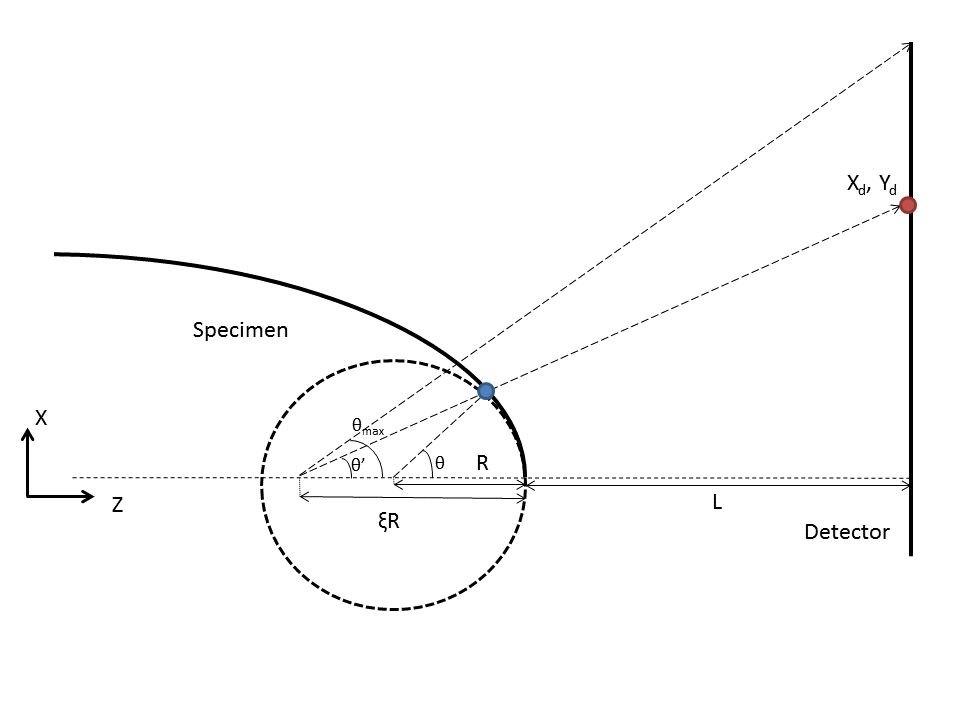
\includegraphics[width=\textwidth]{p3_projection}
	}
	\caption{Схема стереографической проекции координат атома на вершину образца \cite{scbibDensity}. Показано определение реального угла испарения иона $\theta$ и наблюдаемого угла испарения иона $\theta$'.}
	\label{fig:p3_projection}
\end{figure} 

Угол $\theta$' рассчитывается по известным значениям расстояния между образцом и детектором и значениями координат иона на детекторе $X_p, Y_p$. Прямая связь между двумя углами $\theta$ и $\theta$' и координатой Z может быть получена как:

\begin{equation}
	\label{eq:equation3_4}
	\theta = \theta' + \arcsin(\xi - 1)\sin{\theta'},
\end{equation}

\begin{equation}
	\label{eq:equation3_5}
	z_i = \frac{\Omega N_i}{Q R^2 \pi 2 {\sin^2(\theta_{max})}} + R (1- \cos{\theta}),
\end{equation}

где $\theta$ - исходный угол вылета иона, который представляет собой реальный угол проекции, $\theta$' - угол, наблюдаемый после сжатия траекторий иона, $\xi$ - фактор сжатия изображения ICF, Q - эффективность обнаружения, $N_i$ - номер обнаруженного атома. Угол $\theta_{max}$ - это максимальный угол обнаружения атомов. Важно отметить, что углы $\theta$ и $\theta$' могут изменяться в пределах от 0 до $\pi/2$.

Далее рассмотрим влияние $k_f$ и ICF на характер изменения координат X, Y и Z более детально. Из выражений \cref{eq:equation3_1,eq:equation3_2,eq:equation3_4} видно, что координаты X и Y  пропорциональны величине ICF в пределах допустимых значений угла $\theta$ от 0 до $\pi/2$. В выражении \cref{eq:equation3_5} Z координата равна сумме двух слагаемых. Первое отвечает за смещение по оси Z вдоль всего образца в зависимости от номера испаренного атома. Второе слагаемое определяется степенью кривизны поверхности, с которой был испарен атом. Фактор сжатия изображения фигурирует только в части определения кривизны поверхности образца. Соответственно, смещение атома по координате Z практически не зависит от ICF. Полевой фактор, в свою очередь, влияет и на координаты X, Y, и на координату Z, поскольку $k_f$ присутствует в формуле определения радиуса~\cref{eq:equation11}.

Для наглядной демонстрации характера зависимостей координат атомов от $k_f$ и ICF был восстановлен один и тот же объем атомов при различных значениях $k_f$ и ICF. На Рисунке \cref{fig:p3_3Dparts} показаны атомные карты образца, восстановленные при разных параметрах восстановления.

\begin{figure}[htb]
	\centerfloat{
		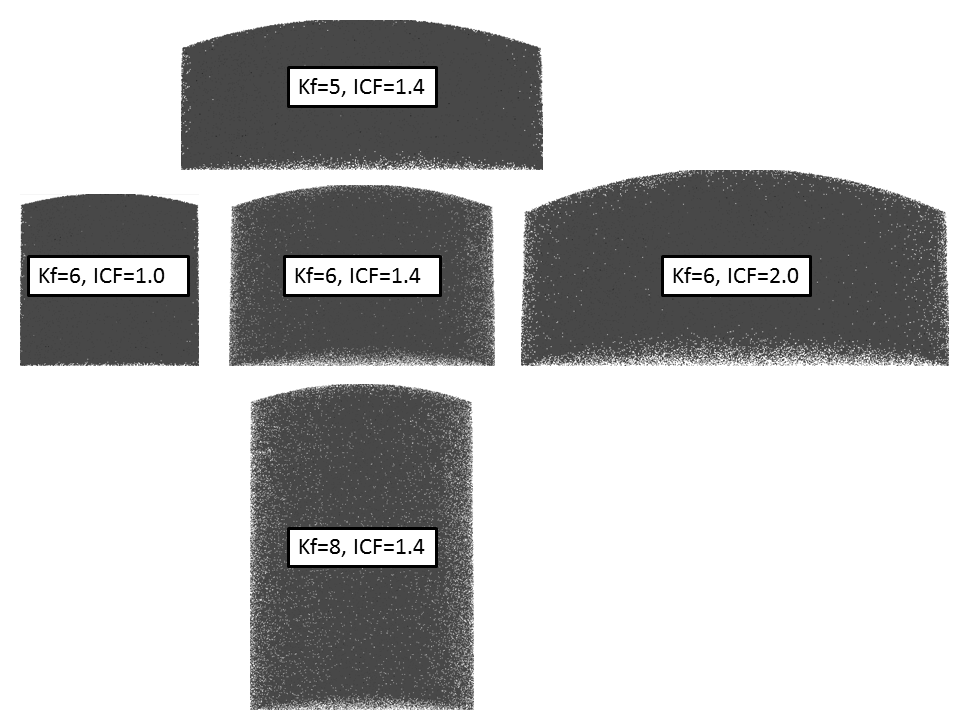
\includegraphics[width=\textwidth]{p3_3Dparts}
	}
	\caption{Атомные карты реконструируемого образца с различными значениях полевого фактора ($k_f$) и фактора сжатия изображения (ICF) \cite{scbibDensity}}
	\label{fig:p3_3Dparts}
\end{figure}

На Рисунке \cref{fig:p3_3Dparts} видно, что при неизменном $k_f$, ICF  влияет только на X, Y координаты и на кривизну поверхности образца. Общая высота образца остается практически низменной. В свою очередь, при постоянном ICF, полевой фактор значительно изменяет все линейные размеры реконструируемого объема. В работе \cite{scbibDensity} было высказано предположение, что изменение полевого фактора не меняет плотность атомов при восстановлении данных. Для проверки данного предположения можно рассчитать значения плотности атомов при различных значения полевого фактора и фактора сжатия изображения (см.~Рисунок~\cref{fig:p3_ICF}).

\begin{figure}[htb]
	\begin{minipage}[b][][b]{0.49\textwidth}\centering
		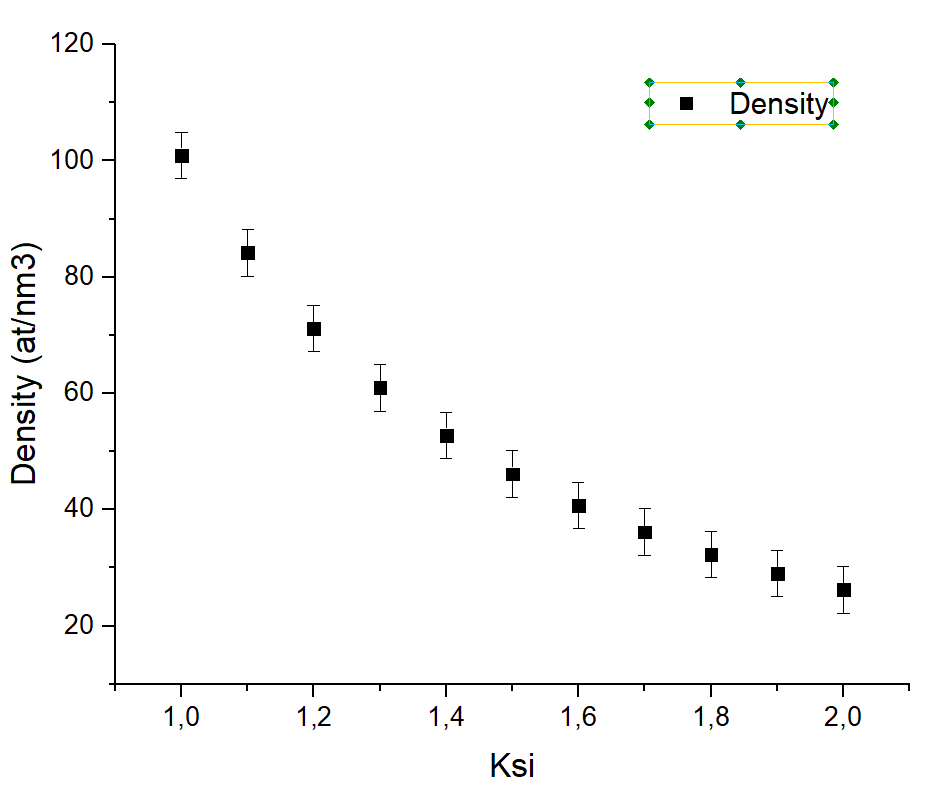
\includegraphics[width=\textwidth]{p3_ICFvsKsi} \\ а)
	\end{minipage}
	%\hfill
	\begin{minipage}[b][][b]{0.49\textwidth}\centering
		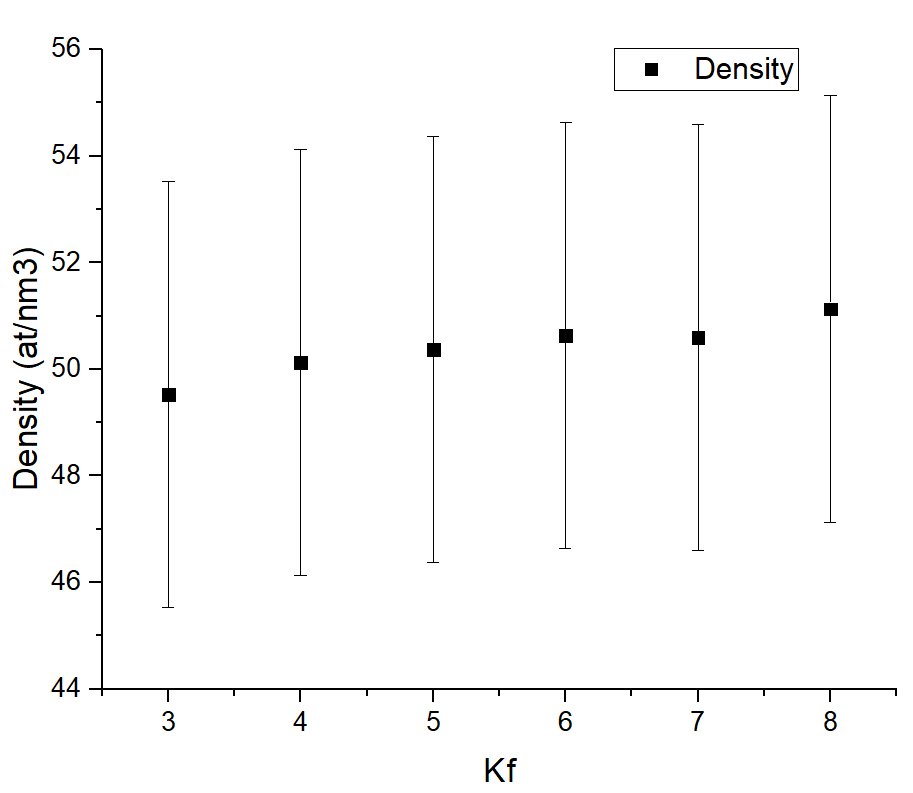
\includegraphics[width=\textwidth]{p3_ICFvskf} \\ б)
	\end{minipage}
	\caption{Значения плотности при различных значениях ICF (а). Значения плотности атомов при различных значениях $k_f$ (б) \cite{scbibDensity}}
	\label{fig:p3_ICF}
\end{figure}

Исходя из допущения, что исследуемый материал имеет постоянную плотность вещества, то есть не имеет включений или объемная доля включений невелика, то плотность атомов можно принять как постоянную величину для всего исследуемого объема. Далее, опираясь на методику определения точности восстановления координат из Раздела \cref{sec:ch3/sect1}, можно рассмотреть следующую методику поиска зависимостей ICF и $k_f$:

\begin{enumerate}[beginpenalty=10000] % https://tex.stackexchange.com/a/476052/104425
	\item Допустим, что плотность атомов постоянна и известна заранее для исследуемого материала, также считаем, что расстояния между атомными плоскостями, соответствующие одному кристаллографическому выходу, постоянны и известны;
	\item Зная плотность атомов подбираем такое значение ICF, чтобы плотность реконструируемого объема совпадала с известной плотностью;
	\item Полевой фактор определяем исходя из трех возможных вариантов:
	\begin{itemize} [beginpenalty=10000]
		\item Если в исследуемом объеме присутствуют включения, и форма этих включений известна (например, зоны Гинье-Престона), то $k_f$ выбирается, так, чтобы форма включений соответствовала ожидаемой;
		\item Если в исследуемом объеме нет включений, то $k_f$ выбирается близким к значениям полевого фактора, выбранных в аналогичных исследованиях;
		\item Если в исследуемом объеме можно различить атомные плоскости, то $k_f$ выбирается таким, чтобы расстояния между атомными плоскостями были одинаковыми во всем объеме данных и наиболее близки к табличному значению.
	\end{itemize}
\end{enumerate}

Стоит отметить, что согласно работам групп Gault \cite{Gault11_Loi}, Loi \cite{Loi13} и Da Costa \cite{Hatzoglou19}, можно предположить, что ICF и $k_f$, найденные для чистых материалов (в которых возможна калибровка по межплоскостным расстояниям), будут одинаковыми для соответствующих сплавов.

Для экспериментального определения значений полевого фактора и фактора сжатия изображений были проведены калибровочные исследования. АЗТ анализ проводился на установке ПАЗЛ-3D. В качестве материалов для исследования выбраны алюминий и вольфрам с объемноцентрированной и гранецентрированной кубической кристаллической структурой соответственно. Исследования проводились при следующих условиях:
\begin{itemize}
	\item температура образца 22 К;
	\item скорость сбора данных от 2 до 6 атомов на 1000 лазерных импульсов;
	\item энергия лазерного импульса от 5 до 10 мВт;
	\item частота лазерных импульсов 25 кГц;
	\item длина волны лазера 515 нм.
\end{itemize} 

Режим испарения поддерживался согласно методике описанной в работе Разницына \cite{scbibOptParamsYAFI}. Реконструкция данных проводилась с помощью программы <<КВАНТМ-3D>> версии 1.5.7. При восстановлении масс-спектра использовалась процедура автоматической калибровки и оптимизации \cite{Shutov19}. Исследования и проверка работоспособности методики проводились на 12 образцах вольфрама и алюминия. Для удобства оценки расстояния между плоскостями атомов был разработан специальный инструмент в программном обеспечении <<KNN-cryst>>. Работа данного инструмента базируется на построении распределения ближайших соседей K порядка \cite{GaultBOOK}, где K принимает значения от 10 до 30 в зависимости от выбора пользователя. <<KNN-cryst>> считает расстояния до ближайших соседей только по Z координате. Ось Z выбрана, поскольку вдоль неё чаще всего наблюдаются атомные плоскости. В случае, если в анализируемом объеме есть атомные плоскости, разработанный инструмент <<увидит>> некоторую периодическую функцию расстояний между ближайшими соседями. Пример показан на Рисунке \cref{fig:p3_atomiccount_distance}. Для визуализации линейной плотности в программе <<КВАНТМ-3D>> модифицирован модуль линейных концентраций. В новой версии возможна визуализация линейной плотности вдоль оси Z, по аналогии с концентрациями, с возможностью выбора шага усреднения и параметров сглаживания.

Для оценки изотропности плотности атомов в объеме рассчитаны значения плотности вдоль оси Z образца алюминия (см. Рисунок \cref{fig:p3_Density_vs_depth}, расчет плотности по стандартному протоколу). 

На Рисунке \cref{fig:p3_Density_vs_depth} видно, что с изменением глубины - меняется значение плотности. Это позволяет предположить, что для корректного восстановления АЗТ данных необходимо внести поправки, связанные с координатой Z, в протокол реконструкции 3D данных. Далее будет описана разработка Протокола динамической реконструкции по плотности материала (ПДРП??). Как выше было сказано, ICF практически не оказывает влияния на Z координату, следовательно, в данном протоколе будет динамически изменяться значение фактора поля.

Исходя из выражений \cref{eq:equation11,eq:equation3_5} и вышеописанных допущений о постоянной плотности, можно заключить, что необходимо найти зависимость полевого фактора от напряжения на образце. Для поиска данной зависимости необходимо разбить объем данных на небольшие части. Для каждой части подобрать такое значение $k_f$, чтобы значение межплоскостных расстояний было наиболее близко к теоретическому. Естественно для калибровки необходимо использовать материал, в котором можно наблюдать атомные плоскости с помощью АЗТ методики. Теоретические значения межплоскостных расстояний можно найти в книге Gault \cite{GaultBOOK}. Из той же книги были использованы карты выходов кристаллографических направлений для определения типа выходов по картам полевого испарения.

\begin{figure}[htb]
	\centerfloat{
		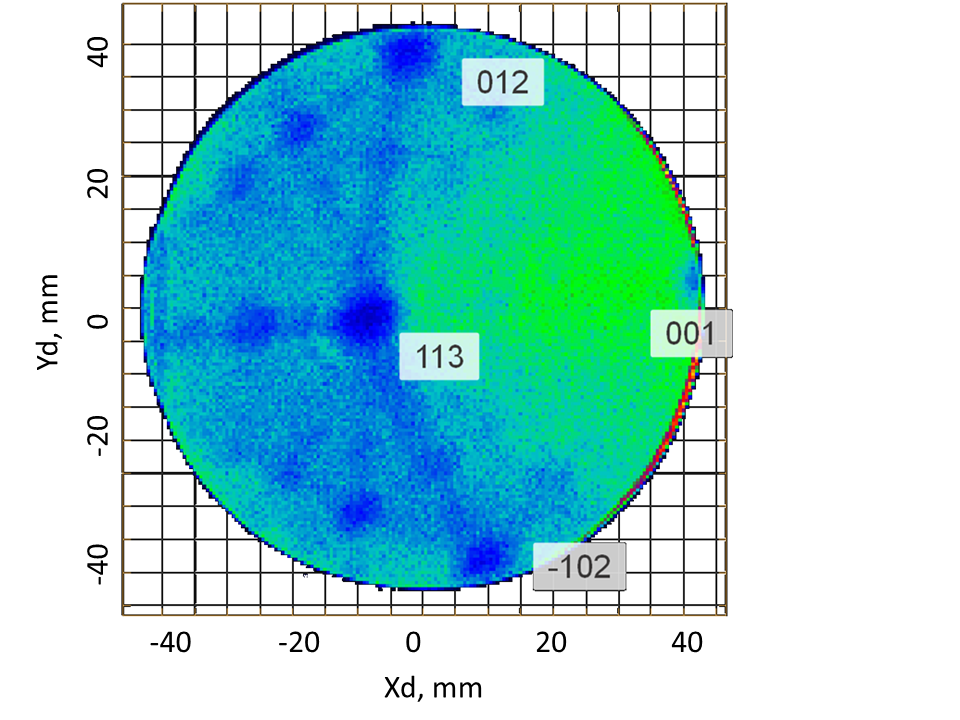
\includegraphics[width=\textwidth]{p3_Alion}
	}
	\caption{Карты полевой десорбции алюминиевого образца. Указаны кристаллографические направления \cite{scbibDensity}}
	\label{fig:p3_Alion}
\end{figure} 

На Рисунке \cref{fig:p3_Alion} показана карта полевого испарения с детектора ПАЗЛ-3D при исследовании алюминиевого образца. Для расчета межплоскостных расстояний был использован выход {113}, поскольку он находится практически в центре детектора, а это значит, что координаты атомов в нем имеют наименьшие искажения. Согласно книге Gault для кристаллографического выхода алюминия {113} расстояние между плоскостями атомов примерно равно 1.2 \r{A}. Выбор разбиения объема на части основывался на требовании получить в каждой части набор из 10-30 плоскостей атомов для более точного определения межплоскостного расстояния. Напряжение для каждой части считалось практически постоянным и равным напряжению в начале сегмента. Полученные значения $k_f$ при различных напряжениях для алюминиевого образца показаны на Рисунке \cref{fig:p3_kf_vs_voltage}. 

\begin{figure}[htb]
	\centerfloat{
		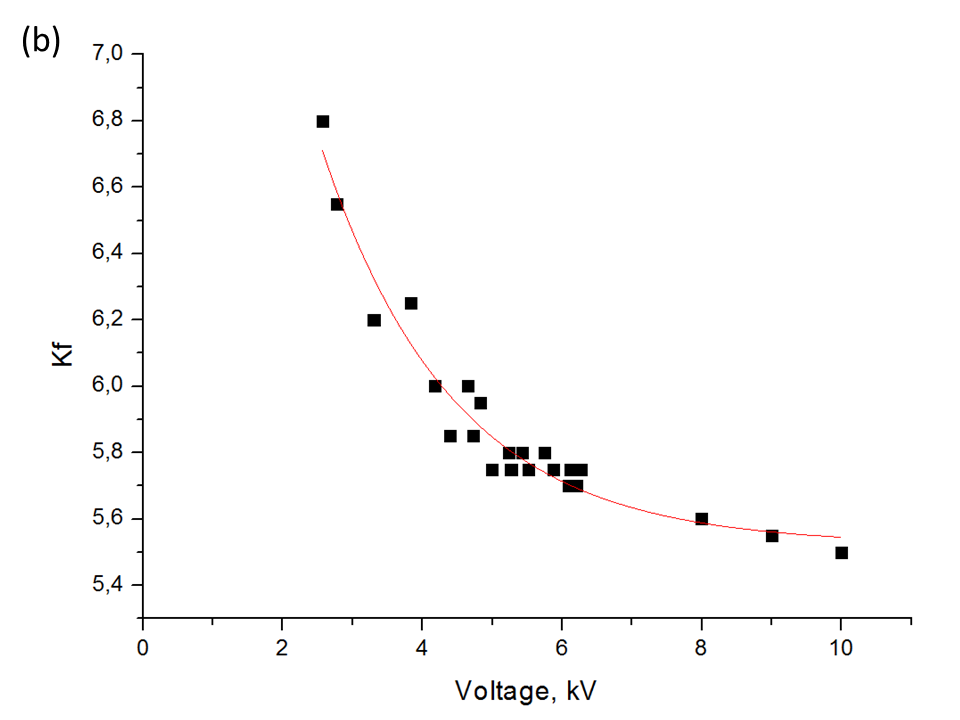
\includegraphics[width=\textwidth]{p3_kf_vs_voltage}
	}
	\caption{Экспериментальные данные $k_f$ \cite{scbibDensity}, полученные для алюминиевого образца (черные точки) и наилучшая аппроксимирующая кривая (красная линия)}
	\label{fig:p3_kf_vs_voltage}
\end{figure} 

Для полученного массива значений $k_f$ и напряжений была проведена аппроксимация экспоненциальной функцией:

\begin{equation}
	\label{eq:equation3_n}
	k_f = (10 - C) + Ce^{-5.3 U 10^{-4}},
\end{equation} 

где C - константа подгонки, U - напряжение на образце. Похожая функция использовалась в работах \cite{Hatzoglou19} и \cite{Loi13}. Различия в зависимостях, возможно, обусловлено различным электростатическим окружением образца в разных установках атомно-зондовой томографии. Значение подгоночной константы для алюминия равно 5.5, а для вольфрама - 4.5. Значимых зависимостей полевого фактора от угла раствора образца или начальным радиусом вершины образца не обнаружено. На Рисунке \cref{fig:p3_PlanesDistance_depth} показаны значения межплоскостных расстояний рассчитанные при использовании разных протоколов реконструкции данных для образца из алюминия. Видно, что  расстояния между плоскостями атомов,  полученные с помощью предлагаемого динамического протокола восстановления, довольно точно совпадают с теоретическим значение.

\begin{figure}[htb]
	\centerfloat{
		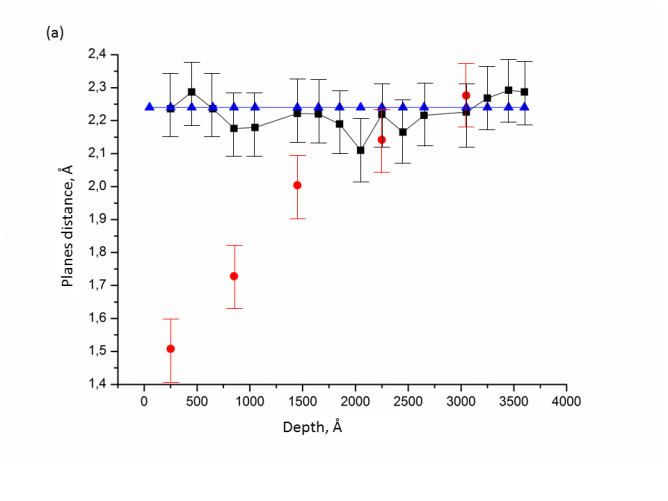
\includegraphics[width=\textwidth]{p3_PlanesDistance_depth}
	}
	\caption{Значения расстояний между атомными плоскостями в зависимости от глубины по оси Z образца из алюминия \cite{scbibDensity}, полученное стандартным протоколом реконструкции (красный), динамическим протоколом $k_f$ (черный). Синим отмечено теоретическое значение межплоскостного расстояния алюминия.}
	\label{fig:p3_PlanesDistance_depth}
\end{figure}

Как выше было указанно, значение ICF влияет на плотность атомов в реконструируемом объеме. Следовательно, определить значение фактора сжатия изображения можно с помощью простого перебора диапазона допустимых значений ICF, с последующим выбором наиболее близкого значения к теоретическому. Допустимые значения ICF находятся в диапазоне от 1 до 2 отн.ед. Для более точного определения значений ICF в зависимости от напряжения на образце необходимо проделать туже процедуру, что и для поиска $k_f$. Объем данных делится по оси Z на небольшие части, для каждой из них методом перебора находится оптимальное значение ICF. В результате был получен набор значений фактора сжатия изображений и напряжений, который аппроксимировался линейной зависимостью. Полученный характер зависимости отличается аналогичных зависимостей, полученных в работах \cite{Hatzoglou19, Gault11_Loi}. Данное отличие связано с использованием разных типов испарения в установках атомно-зондовой томографии. В ПАЗЛ-3D используется лазерное испарение, а в аналогичных работах используются установки с лазерным испарением и/или локальным электродом.

На Рисунке \cref{fig:p3_Density_vs_depth} показаны значения плотности каждой части объема в зависимости от положения по оси Z образца из алюминия. Видно, что с помощью Протокола динамической реконструкции по плотности материала (ПДРП??) удалось нивелировать понизительную тенденцию в реконструкции данных. При это сохраняются отклонения плотности атомов от целевого значения на значимые величины. Предположительно это связано с не идеальной формой кончика образца.

\begin{figure}[htb]
	\centerfloat{
		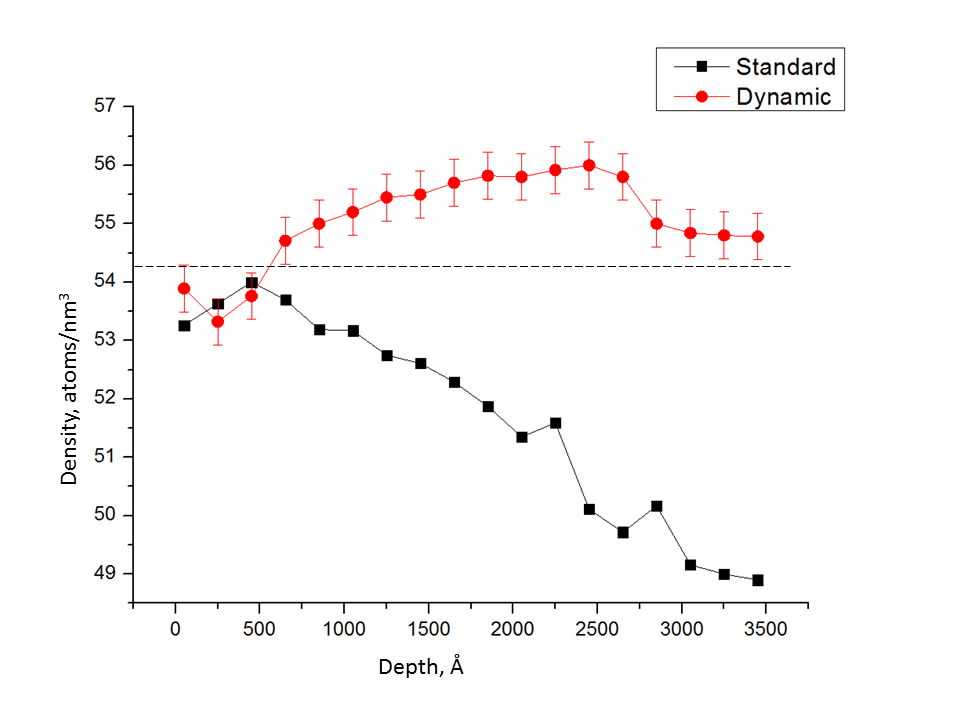
\includegraphics[width=\textwidth]{p3_Density_vs_depth}
	}
	\caption{Значения линейной плотности атомов в образце из алюминия вдоль оси Z образца \cite{scbibDensity}, полученная по стандартному протоколу (черные точки) и по Протоколу динамической реконструкции по плотности материала (ПДРП??) (красные точки). Пунктирная линия показывает ожидаемую плотность алюминия.}
	\label{fig:p3_Density_vs_depth}
\end{figure}

Для оценки качества работы Протокола динамической реконструкции по плотности материала (ПДРП??) построено распределение расстояний между атомами вдоль оси Z с помощью инструмента <<KNN-cryst>>. На Рисунке \cref{fig:p3_atomiccount_distance} видно, что ошибка определения координаты Z для атомов накапливается с увеличением расстояния вдоль оси Z. В случае среднестатистического размера исследуемой области в 
образце от 100 до 1000 нм для атомно-зондовой томографии ошибка значения координаты Z может достигать 50\%. Предложенный протокол позволит точнее определять размеры исследуемой области и размеры больших фаз и включений.

\begin{figure}[htb]
	\centerfloat{
		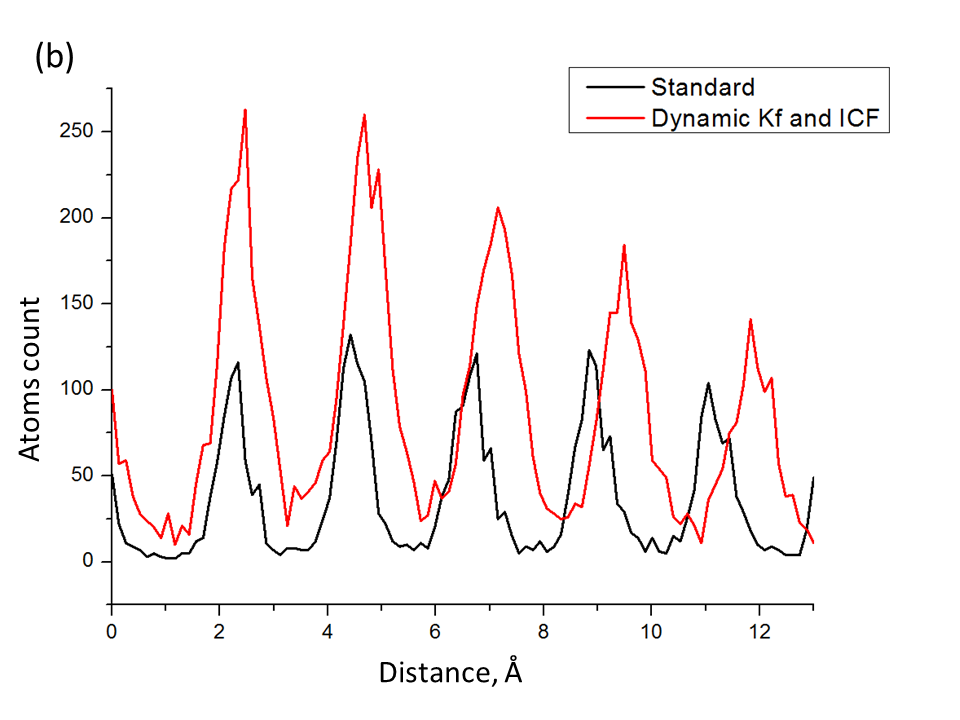
\includegraphics[width=\textwidth]{p3_atomiccount_distance}
	}
	\caption{Распределение расстояний между атомами \cite{scbibDensity}.}
	\label{fig:p3_atomiccount_distance}
\end{figure}


%\subsection{Подпараграф \cyrdash{} два}\label{subsec:ch3/sect33/sub2}

%Некоторый текст.

\FloatBarrier
\section{Основные результаты по главе 3}\label{sec:ch3/sect6}

Для разработанной установки были проведены исследования, подтверждающие её характеристики в части пространственного разрешения ( и разрешения по массе).

Проведена работа по определению оптимальной метрики качества АЗТ данных. Рассмотрен набор метрик-кандидатов: ...... 
Выбрана метрика  - отношение количества ионов с разной зарядностью. Данная метрика обеспечивает наилучшую воспроизводимость результатов исследований. 

Проведено сравнение условий испарения на разных атомно-зондовых томографах. Показана возможность получать совпадающие,в пределах погрешности, данные о составе и структуре материалов на разных установках АЗТ.

Определены зависимости параметров восстановления данных от испаряющего напряжения для алюминия и вольфрама. На основе полученных зависимостей предложен оригинальный протокол динамической реконструкции по плотности материал. Данная методика позволяет существенно сократить ошибку определения 3D координат атомов в больших объемах данных.










\clearpage
